% Options for packages loaded elsewhere
\PassOptionsToPackage{unicode}{hyperref}
\PassOptionsToPackage{hyphens}{url}
%
\documentclass[
]{book}
\usepackage{amsmath,amssymb}
\usepackage{iftex}
\ifPDFTeX
  \usepackage[T1]{fontenc}
  \usepackage[utf8]{inputenc}
  \usepackage{textcomp} % provide euro and other symbols
\else % if luatex or xetex
  \usepackage{unicode-math} % this also loads fontspec
  \defaultfontfeatures{Scale=MatchLowercase}
  \defaultfontfeatures[\rmfamily]{Ligatures=TeX,Scale=1}
\fi
\usepackage{lmodern}
\ifPDFTeX\else
  % xetex/luatex font selection
\fi
% Use upquote if available, for straight quotes in verbatim environments
\IfFileExists{upquote.sty}{\usepackage{upquote}}{}
\IfFileExists{microtype.sty}{% use microtype if available
  \usepackage[]{microtype}
  \UseMicrotypeSet[protrusion]{basicmath} % disable protrusion for tt fonts
}{}
\makeatletter
\@ifundefined{KOMAClassName}{% if non-KOMA class
  \IfFileExists{parskip.sty}{%
    \usepackage{parskip}
  }{% else
    \setlength{\parindent}{0pt}
    \setlength{\parskip}{6pt plus 2pt minus 1pt}}
}{% if KOMA class
  \KOMAoptions{parskip=half}}
\makeatother
\usepackage{xcolor}
\usepackage{color}
\usepackage{fancyvrb}
\newcommand{\VerbBar}{|}
\newcommand{\VERB}{\Verb[commandchars=\\\{\}]}
\DefineVerbatimEnvironment{Highlighting}{Verbatim}{commandchars=\\\{\}}
% Add ',fontsize=\small' for more characters per line
\usepackage{framed}
\definecolor{shadecolor}{RGB}{248,248,248}
\newenvironment{Shaded}{\begin{snugshade}}{\end{snugshade}}
\newcommand{\AlertTok}[1]{\textcolor[rgb]{0.94,0.16,0.16}{#1}}
\newcommand{\AnnotationTok}[1]{\textcolor[rgb]{0.56,0.35,0.01}{\textbf{\textit{#1}}}}
\newcommand{\AttributeTok}[1]{\textcolor[rgb]{0.13,0.29,0.53}{#1}}
\newcommand{\BaseNTok}[1]{\textcolor[rgb]{0.00,0.00,0.81}{#1}}
\newcommand{\BuiltInTok}[1]{#1}
\newcommand{\CharTok}[1]{\textcolor[rgb]{0.31,0.60,0.02}{#1}}
\newcommand{\CommentTok}[1]{\textcolor[rgb]{0.56,0.35,0.01}{\textit{#1}}}
\newcommand{\CommentVarTok}[1]{\textcolor[rgb]{0.56,0.35,0.01}{\textbf{\textit{#1}}}}
\newcommand{\ConstantTok}[1]{\textcolor[rgb]{0.56,0.35,0.01}{#1}}
\newcommand{\ControlFlowTok}[1]{\textcolor[rgb]{0.13,0.29,0.53}{\textbf{#1}}}
\newcommand{\DataTypeTok}[1]{\textcolor[rgb]{0.13,0.29,0.53}{#1}}
\newcommand{\DecValTok}[1]{\textcolor[rgb]{0.00,0.00,0.81}{#1}}
\newcommand{\DocumentationTok}[1]{\textcolor[rgb]{0.56,0.35,0.01}{\textbf{\textit{#1}}}}
\newcommand{\ErrorTok}[1]{\textcolor[rgb]{0.64,0.00,0.00}{\textbf{#1}}}
\newcommand{\ExtensionTok}[1]{#1}
\newcommand{\FloatTok}[1]{\textcolor[rgb]{0.00,0.00,0.81}{#1}}
\newcommand{\FunctionTok}[1]{\textcolor[rgb]{0.13,0.29,0.53}{\textbf{#1}}}
\newcommand{\ImportTok}[1]{#1}
\newcommand{\InformationTok}[1]{\textcolor[rgb]{0.56,0.35,0.01}{\textbf{\textit{#1}}}}
\newcommand{\KeywordTok}[1]{\textcolor[rgb]{0.13,0.29,0.53}{\textbf{#1}}}
\newcommand{\NormalTok}[1]{#1}
\newcommand{\OperatorTok}[1]{\textcolor[rgb]{0.81,0.36,0.00}{\textbf{#1}}}
\newcommand{\OtherTok}[1]{\textcolor[rgb]{0.56,0.35,0.01}{#1}}
\newcommand{\PreprocessorTok}[1]{\textcolor[rgb]{0.56,0.35,0.01}{\textit{#1}}}
\newcommand{\RegionMarkerTok}[1]{#1}
\newcommand{\SpecialCharTok}[1]{\textcolor[rgb]{0.81,0.36,0.00}{\textbf{#1}}}
\newcommand{\SpecialStringTok}[1]{\textcolor[rgb]{0.31,0.60,0.02}{#1}}
\newcommand{\StringTok}[1]{\textcolor[rgb]{0.31,0.60,0.02}{#1}}
\newcommand{\VariableTok}[1]{\textcolor[rgb]{0.00,0.00,0.00}{#1}}
\newcommand{\VerbatimStringTok}[1]{\textcolor[rgb]{0.31,0.60,0.02}{#1}}
\newcommand{\WarningTok}[1]{\textcolor[rgb]{0.56,0.35,0.01}{\textbf{\textit{#1}}}}
\usepackage{longtable,booktabs,array}
\usepackage{calc} % for calculating minipage widths
% Correct order of tables after \paragraph or \subparagraph
\usepackage{etoolbox}
\makeatletter
\patchcmd\longtable{\par}{\if@noskipsec\mbox{}\fi\par}{}{}
\makeatother
% Allow footnotes in longtable head/foot
\IfFileExists{footnotehyper.sty}{\usepackage{footnotehyper}}{\usepackage{footnote}}
\makesavenoteenv{longtable}
\usepackage{graphicx}
\makeatletter
\def\maxwidth{\ifdim\Gin@nat@width>\linewidth\linewidth\else\Gin@nat@width\fi}
\def\maxheight{\ifdim\Gin@nat@height>\textheight\textheight\else\Gin@nat@height\fi}
\makeatother
% Scale images if necessary, so that they will not overflow the page
% margins by default, and it is still possible to overwrite the defaults
% using explicit options in \includegraphics[width, height, ...]{}
\setkeys{Gin}{width=\maxwidth,height=\maxheight,keepaspectratio}
% Set default figure placement to htbp
\makeatletter
\def\fps@figure{htbp}
\makeatother
\setlength{\emergencystretch}{3em} % prevent overfull lines
\providecommand{\tightlist}{%
  \setlength{\itemsep}{0pt}\setlength{\parskip}{0pt}}
\setcounter{secnumdepth}{5}
\usepackage{booktabs}

\usepackage{graphicx}
\usepackage{fontspec} % For Unicode support
\graphicspath{{images/}}

\ifLuaTeX
  \usepackage{selnolig}  % disable illegal ligatures
\fi
\usepackage[]{natbib}
\bibliographystyle{plainnat}
\usepackage{bookmark}
\IfFileExists{xurl.sty}{\usepackage{xurl}}{} % add URL line breaks if available
\urlstyle{same}
\hypersetup{
  pdftitle={Untitled},
  pdfauthor={Dr Mostafa},
  hidelinks,
  pdfcreator={LaTeX via pandoc}}

\title{Untitled}
\author{Dr Mostafa}
\date{2025-03-05}

\begin{document}
\maketitle

{
\setcounter{tocdepth}{2}
\tableofcontents
}
\chapter*{About The Workbook}\label{about-the-workbook}

This is a \emph{worksheet} written in \textbf{Markdown}. It shows the question and answers of the MATH224 workbook.

\chapter*{Table of Contents}\label{table-of-contents}

\phantomsection\label{toc}
Module 1:

Introduction to Data

1.1 Summarizing Numerical Data

1.2 Summarizing Categorical Data

Module 2:

Probability Rules

2.1 Review on Probability

2.2 Random Variables

2.3 Binomial Distribution

2.4 Normal Distribution

Module 3:

Inference For Proportion

3.1 Point Estimate

3.2 Confidence Interval

Module 4:

Inference For Mean

4.1 Review on Inference for Mean

4.2 Central Limit Theorem

Module 5:

Linear Regression

5.1 Introduction to Linear Regression

\chapter{Introduction to Data}\label{introduction-to-data}

\textbf{Objective 1:} By the end of this unit, students will be able to:

\begin{itemize}
\tightlist
\item
  Understand the importance of statistical methods for answering research questions using data.
\item
  Identify different types of data that can be analyzed using statistical methods.
\item
  Describe basic sampling principles and strategies for the purpose of collecting data for research studies.
\item
  Describe basic principles of designing research experiments.
\end{itemize}

\section{Quick Review of the Data}\label{quick-review-of-the-data}

\begin{enumerate}
\def\labelenumi{\arabic{enumi}.}
\tightlist
\item
  Compute different proportions in different groups
\end{enumerate}

\begin{itemize}
\tightlist
\item
  For example, treatment group(s) and control group(s), (these are also called as conditional probabilities in later discussions)
\end{itemize}

\begin{enumerate}
\def\labelenumi{\arabic{enumi}.}
\setcounter{enumi}{1}
\tightlist
\item
  Data basics
\end{enumerate}

\begin{itemize}
\tightlist
\item
  Types of variables---Numerical (quantitative), Categorical (qualitative);
\item
  Explanatory and response variables;
\item
  Associated (dependent) variables, positive/negative association
\end{itemize}

\begin{enumerate}
\def\labelenumi{\arabic{enumi}.}
\setcounter{enumi}{2}
\tightlist
\item
  Sampling:
\end{enumerate}

\begin{enumerate}
\def\labelenumi{\arabic{enumi})}
\item
  Identify the research question (then determine the population)
\item
  Collect data that are reliable and help achieve the research goal (take good samples)
\end{enumerate}

\begin{itemize}
\item
  Population and sample

  \begin{itemize}
  \tightlist
  \item
    A population is the entire group that you want to draw conclusions about.
  \item
    A sample is the specific group that you will collect data from
  \end{itemize}
\item
  Parameter and Statistic

  \begin{itemize}
  \tightlist
  \item
    A descriptive measure (for example, average, median, standard deviation and percentages) for an entire population is a '\,`\textbf{parameter.}'\,'
  \item
    A descriptive measure for a sample is referred to as a '\,`\textbf{sample statistic}'\,'
  \end{itemize}
\item
  Observational studies and Experiments

  \begin{itemize}
  \tightlist
  \item
    Observational studies: research processes where researchers collect data in a way that does not directly interfere with how the data arise (examine something without manipulating it)
  \item
    Experiment: Researchers randomly assign subjects to various treatments in order to establish causal connections between the explanatory and response variables
  \end{itemize}
\item ~
  \section{Four commonly used random sampling techniques:}\label{four-commonly-used-random-sampling-techniques}

\begin{verbatim}
1.  Simple random sampling
\end{verbatim}

  \begin{itemize}
  \tightlist
  \item
    \begin{enumerate}
    \def\labelenumi{\arabic{enumi}.}
    \setcounter{enumi}{1}
    \tightlist
    \item
      Stratified sample
    \end{enumerate}
  \item
    \begin{enumerate}
    \def\labelenumi{\arabic{enumi}.}
    \setcounter{enumi}{2}
    \tightlist
    \item
      Cluster sampling
    \end{enumerate}
  \item
    \begin{enumerate}
    \def\labelenumi{\arabic{enumi}.}
    \setcounter{enumi}{3}
    \tightlist
    \item
      Multistage sampling
    \end{enumerate}
  \end{itemize}
\end{itemize}

\begin{enumerate}
\def\labelenumi{\arabic{enumi}.}
\setcounter{enumi}{3}
\tightlist
\item
  Principles of experimental design: 4 principles
\end{enumerate}

\begin{itemize}
\tightlist
\item
  Controlling (assign treatment and control groups, enforce specific treatment in treatment group)
\item
  Randomization (randomly assign treatment group and control group);
\item
  Replication (large sample, or replicate an entire study to verify earlier findings)
\item
  Blocking
\end{itemize}

\textbf{Exercise 1.} (page 11 \#1.2) Researchers studying the effect of antibiotic treatment for acute sinusitis compared to symptomatic treatments randomly assigned 166 adults diagnosed with acute sinusitis to one of two groups: treatment or control. Study participants received either a 10-day course of amoxicillin (an antibiotic) or a placebo similar in appearance and taste. The placebo consisted of symptomatic treatments such as acetaminophen nasal decongestants, etc. At the end of the 10-day period, patients were asked if they experienced improvement in symptoms. The distribution of responses is summarized below (with some cells missing numbers):

\emph{(for b), c), Round answers to within one hundredth of a percent)}

\begin{longtable}[]{@{}
  >{\raggedright\arraybackslash}p{(\columnwidth - 8\tabcolsep) * \real{0.1667}}
  >{\raggedright\arraybackslash}p{(\columnwidth - 8\tabcolsep) * \real{0.3333}}
  >{\raggedright\arraybackslash}p{(\columnwidth - 8\tabcolsep) * \real{0.1667}}
  >{\raggedright\arraybackslash}p{(\columnwidth - 8\tabcolsep) * \real{0.1667}}
  >{\raggedright\arraybackslash}p{(\columnwidth - 8\tabcolsep) * \real{0.1667}}@{}}
\toprule\noalign{}
\begin{minipage}[b]{\linewidth}\raggedright
\end{minipage} & \begin{minipage}[b]{\linewidth}\raggedright
Self-reported improved in symptoms
\end{minipage} & \begin{minipage}[b]{\linewidth}\raggedright
\end{minipage} & \begin{minipage}[b]{\linewidth}\raggedright
\end{minipage} & \begin{minipage}[b]{\linewidth}\raggedright
\end{minipage} \\
\midrule\noalign{}
\endhead
\bottomrule\noalign{}
\endlastfoot
& & \textbf{Yes} & \textbf{No} & \textbf{Total} \\
\textbf{Treatment} & & 66 & & 85 \\
\textbf{Control} & & 65 & & \\
\textbf{Total} & & & & 166 \\
\end{longtable}

(a). Fill the blank cells in the above table.

(b). What percent of patients in the treatment group experienced improvement in symptoms?

(c). What percent experienced improvement in symptoms in the control group?

(d). In which group did a higher percentage of patients experience improvement in symptoms?

(e). Your findings so far might suggest a real difference in effectiveness of antibiotic and placebo treatments for improving symptoms of sinusitis. However, this is not the only possible conclusion that can be drawn based on your findings so far. What is one other possible explanation for the observed difference between the percentages of patients in the antibiotic and placebo treatment groups that experience improvement in symptoms of sinusitis?

\textbf{(Answers for reference:}

\textbf{(a).}

\begin{longtable}[]{@{}
  >{\raggedright\arraybackslash}p{(\columnwidth - 8\tabcolsep) * \real{0.1667}}
  >{\raggedright\arraybackslash}p{(\columnwidth - 8\tabcolsep) * \real{0.3333}}
  >{\raggedright\arraybackslash}p{(\columnwidth - 8\tabcolsep) * \real{0.1667}}
  >{\raggedright\arraybackslash}p{(\columnwidth - 8\tabcolsep) * \real{0.1667}}
  >{\raggedright\arraybackslash}p{(\columnwidth - 8\tabcolsep) * \real{0.1667}}@{}}
\toprule\noalign{}
\begin{minipage}[b]{\linewidth}\raggedright
\end{minipage} & \begin{minipage}[b]{\linewidth}\raggedright
Self-reported improved in symptoms
\end{minipage} & \begin{minipage}[b]{\linewidth}\raggedright
\end{minipage} & \begin{minipage}[b]{\linewidth}\raggedright
\end{minipage} & \begin{minipage}[b]{\linewidth}\raggedright
\end{minipage} \\
\midrule\noalign{}
\endhead
\bottomrule\noalign{}
\endlastfoot
& & \textbf{Yes} & \textbf{No} & \textbf{Total} \\
\textbf{Treatment} & & 66 & 19 & 85 \\
\textbf{Control} & & 65 & 16 & 81 \\
\textbf{Total} & & 131 & 35 & 166 \\
\end{longtable}

\textbf{(e).} Be careful: Do not generalize the results of this study. It is impossible to tell merely by comparing the sample proportions \textbf{because the difference could be the result of random error in our sample.}

\textbf{Exercise 2.} The following figure displays data from a lending company.

\begin{longtable}[]{@{}
  >{\raggedright\arraybackslash}p{(\columnwidth - 12\tabcolsep) * \real{0.1688}}
  >{\raggedright\arraybackslash}p{(\columnwidth - 12\tabcolsep) * \real{0.1948}}
  >{\raggedright\arraybackslash}p{(\columnwidth - 12\tabcolsep) * \real{0.0779}}
  >{\raggedright\arraybackslash}p{(\columnwidth - 12\tabcolsep) * \real{0.0909}}
  >{\raggedright\arraybackslash}p{(\columnwidth - 12\tabcolsep) * \real{0.0909}}
  >{\raggedright\arraybackslash}p{(\columnwidth - 12\tabcolsep) * \real{0.1818}}
  >{\raggedright\arraybackslash}p{(\columnwidth - 12\tabcolsep) * \real{0.1948}}@{}}
\toprule\noalign{}
\begin{minipage}[b]{\linewidth}\raggedright
loan.amount
\end{minipage} & \begin{minipage}[b]{\linewidth}\raggedright
interest.rate
\end{minipage} & \begin{minipage}[b]{\linewidth}\raggedright
term
\end{minipage} & \begin{minipage}[b]{\linewidth}\raggedright
grade
\end{minipage} & \begin{minipage}[b]{\linewidth}\raggedright
state
\end{minipage} & \begin{minipage}[b]{\linewidth}\raggedright
total.income
\end{minipage} & \begin{minipage}[b]{\linewidth}\raggedright
homeownership
\end{minipage} \\
\midrule\noalign{}
\endhead
\bottomrule\noalign{}
\endlastfoot
7500 & 7.34 & 36 & A & MD & 70000 & rent \\
25000 & 9.43 & 60 & B & OH & 254000 & mortgage \\
14500 & 6.08 & 36 & A & MO & 80000 & mortgage \\
\ldots{} & \ldots{} & \ldots{} & \ldots{} & \ldots{} & \ldots{} & \ldots{} \\
3000 & 7.96 & 36 & A & CA & 34000 & rent \\
\end{longtable}

\textbf{Variable descriptions}

loan amount: Amount of the loan received, in US dollars.

interest rate: Interest rate on the loan, in an annual percentage.

term: The length of the loan, which is always set as a whole number of months.

grade: Loan grade, which takes a values A through G and represents the quality of the loan and its likelihood of being repaid.

state: US state where the borrower resides.

total income: Borrower's total income, including any second income, in US dollars.

homeownership: Indicates whether the person owns, owns but has a mortgage, or rents.

(a). How many cases in the data?

(b). Identify the types of variables.

\textbf{Exercise 3.} (page 19 \#1.4) The Buteyko method is a shallow breathing technique developed by Konstantin Buteyko, a Russian doctor, in 1952. Anecdotal evidence (evidence based only on personal observation) suggests that the Buteyko method can reduce asthma symptoms and improve quality of life. In a scientific study to determine the effectiveness of this method, researchers recruited 600 asthma patients aged 18-69 who relied on medication for asthma treatment. These patients were randomly split into two research groups: one practiced the Buteyko method and the other did not. Patients were scored on quality of life, activity, asthma symptoms, and medication reduction on a scale from 0 to 10. On average, the participants in the Buteyko group experienced a significant reduction in asthma symptoms and an improvement in quality of life.

(a). Identify the main research question of the study.

(b). Who are the subjects in this study and how many are included?

(c). What are the variables in the study? Identify each variable as numerical or categorical. If numerical, state whether the variable is discrete or continuous.

(Reference answer:

(a). The effect of Buteyko method on reducing asthma symptoms and improving quality of life.

(b). Asthma patients aged 18-69 who relied on medication for asthma treatment; 600.

(c). The variables and types are: quality of life (categorical), activity (categorical), asthma symptoms (categorical), and medication reduction on a scale from 0 to 10 (numerical discrete).)

\textbf{Exercise 4.} (page 29 \#1.13) Exercise 1.3 introduces a study where researchers collected data to examine the relationship between air pollutants and preterm births in Southern California. During the study, air pollution levels were measured by air quality monitoring stations; lengths of gestation data were collected on 143,196 births between the years 1989 and 1993; and air pollution exposure during gestation was calculated for each birth.

(a). Identify the population of interest and the sample in this study.

(b). Comment on whether or not the results of the study can be generalized to the population and if the findings of the study can be used to establish causal relationships.

(Reference answer:

\begin{enumerate}
\def\labelenumi{(\alph{enumi})}
\item
  Population: all births in Southern California. Sample: collected length of gestation data of 143,196 births between the years 1989 and 1993.
\item
  If the collected lengths of gestation data of births in this time span and geography can be considered representative of all births, then the results are generalizable to the population of Southern California. However, since the study is observational, the findings cannot be used to establish causal relationships.)
\end{enumerate}

\textbf{Exercise 5.} A fitness center is interested in the average amount of time a client exercises in the center each week. Match the vocabulary words (a-f) with its corresponding examples (1-6). (Note: 1-1 match)

Examples:

\begin{enumerate}
\def\labelenumi{\arabic{enumi}.}
\item
  All 45 exercise times that were recorded from the participants in the study.
\item
  The 45 clients from the fitness center who participated in the study.
\item
  All clients at the fitness center.
\item
  The average amount of time that all clients from the fitness center exercise.
\item
  The amount of time that any given client from the fitness center exercises.
\item
  The average amount of exercise time for the 45 clients from the fitness center who participated in the study.
\end{enumerate}

Vocabulary words:

\begin{enumerate}
\def\labelenumi{\alph{enumi}.}
\item
  Data
\item
  Population
\item
  Variable
\item
  Sample
\item
  Parameter
\item
  Statistic
\end{enumerate}

\textbf{Exercise 6.} (Observational Study or Experiment)

\begin{enumerate}
\def\labelenumi{\alph{enumi}.}
\item
  You would like to investigate whether listening to music while taking exams affects performance. A group of students are told to listen to music while taking a test and their results are compared to a group not listening to music. Is this an experiment or an observational study?
\item
  The starting salaries of recent graduates from Ivy League private and public universities are recorded. Is this an experiment or an observational study?
\end{enumerate}

\textbf{Exercise 7.} (page 37 \#1.41) In a public health study on the effects of consumption of fruits and vegetables on psychological well-being in young adults, participants were randomly assigned to three groups: (1) diet as usual, (2) an ecological momentary intervention involving text message reminders to increase their fruits and vegetable consumption plus a voucher to purchase them, or (3) a fruit and vegetable intervention in which participants were given two additional daily servings of fresh fruits and vegetables to consume on top of their normal diet. Participants were asked to take a nightly survey on their smartphones. Participants were student volunteers at the University of Otago, New Zealand. At the end of the 14-day study, only participants in the third group showed improvements to their psychological well-being across the 14-days relative to the other groups.

(a). What type of study is this?

(b). Identify the explanatory and response variables.

(c). Comment on whether the results of the study can be generalized to the population.

(d). Comment on whether the results of the study can be used to establish causal relationships.

(e). A newspaper article reporting on the study states, ``The results of this study provide proof that giving young adults fresh fruits and vegetables to eat can have psychological benefits even over a brief period of time.'' How would you suggest revising this statement so that it can be supported by the study?

(Reference answer:

(a). Experiment

(b). Explanatory: treatment group (categorical with 3 levels). Response variable: Psychological well-being.

(c). No, because the participants were volunteers.

(d). Yes, because it was an experiment.

(e). The statement should say ``evidence'' instead of ``proof''.)

\newpage

\section{Summarizing Numerical Data}\label{summarizing-numerical-data}

\textbf{Objective 2:} By the end of this unit, students will be able to:

\begin{itemize}
\tightlist
\item
  Summarize and describe numerical data using various visual displays including histograms and dotplots.
\item
  Idnetify skewness in the distribution of numerical data.
\item
  Use summary statistics such as mean and median to describe central tendancy of the data.
\item
  Use summary statistics such as variance, standard deviation, and quartiles to describe variability of the data.
\item
  Identify potential outliers in the data using boxplots.
\end{itemize}

\textbf{Quick Review:}

\textbf{1. Graphical Presentations}

\begin{itemize}
\tightlist
\item
  Scatter graph---present related two numerical data, see if there is any association, outliers
\item
  Dot plot --see overall pattern outliers
\item
  Histogram -- see the shape of data distribution: modals, skewness
\end{itemize}

\textbf{2. Numerical summaries}

\begin{itemize}
\tightlist
\item
  Mean, Median -- both measures are for the center of numerical data
\item
  Mean \(\bar{x} = \frac{1}{n} \sum_{i=1}^{n} x_i\)\\
\item
  Median is the middle value of the arranged data
\item
  Standard Deviation ---measures the spread or variation
\item
  Quartiles, interquartile range,
\item
  Five number summary: Min, Q1, Q2, Q3, Max
\item
  Use the mean and the standard deviation for symmetrical data or large data
\item
  Use the median and interquartile range for skewed data
\end{itemize}

\textbf{3. R functions codes}

\begin{itemize}
\tightlist
\item
  \texttt{c(?,?,?)} -- concatenate function put multiple values in a vector
\item
  \texttt{mean(c(?,?,?))} -- mean
\item
  \texttt{var(c(?,?,?))} -- variance
\item
  \texttt{sd(c(?,?,?))} -- standard deviation
\item
  \texttt{median(c(?,?,?))} -- median
\item
  \texttt{quantile(c(?,?,?),\ quantile.type=2)} \# change type to 6, if n=5
\item
  \texttt{IQR(c(?,?,?),\ quantile.type=2)} \# change type to 6, if n=5
\item
  \texttt{summary(c(?,?,?),\ quantile.type=2)} \# change type to 6, if n=5
\end{itemize}

\textbf{Exercise 1.} Use the following dot plot of an interest rate of some loan data to answer questions.

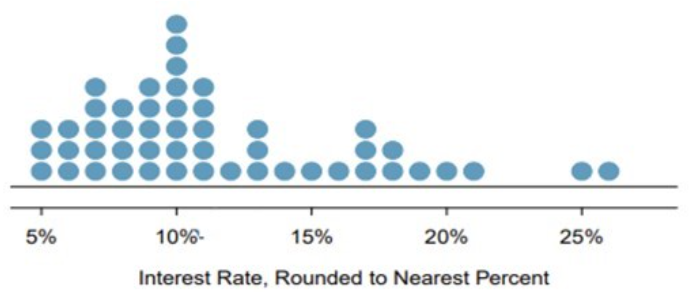
\includegraphics[width=3.66667in,height=\textheight]{images/img23.png}

(a). How many loans?

(b). What is the lowest interest rate? What is the highest interest rate? Find the range.

(c). Find the mean (average).

(d). Find the median.

Help: Using R,

\begin{itemize}
\item
  \texttt{x\ \textless{}-\ c(5,\ 5,\ 5,\ 6,\ 6,\ 6,\ 7,\ 7,\ 7,\ 7,\ 7,\ 8,\ 8,\ 8,\ 8,\ 9,\ 9,\ 9,\ 9,\ 9,\ 10,\ 10,\ 10,\ 10,\ 10,\ 10,\ 10,\ 10,\ 11,\ 11,\ 11,\ 11,\ 11,\ 12,\ 13,\ 13,\ 13,\ 14,\ 15,\ 16,\ 17,\ 17,\ 17,\ 18,\ 118,\ 19,\ 20,\ 21,\ 25,\ 26)}
\item
  \texttt{length(x)}
\item
  \texttt{mean(x)}
\item
  \texttt{median(x)}
\end{itemize}

(Answer: (a) 50 (b) 5; 26; 21 (c) 13.48 (d) 10)

\textbf{Exercise 2.} When we have a distribution where all observations are greater than 0, that is, all \(x_i > 0\), the statistic \(\frac{\text{mean}}{\text{median}}\) can be used as a measure of skewness. What is the expected shape of the distribution under the following conditions? Sketch the shape to illustrate.

\begin{enumerate}
\def\labelenumi{(\alph{enumi})}
\item
  \(\frac{\text{mean}}{\text{median}} = 1\)
\item
  \(\frac{\text{mean}}{\text{median}} < 1\)
\item
  \(\frac{\text{mean}}{\text{median}} > 1\)
\end{enumerate}

\textbf{Exercise 3.} For given two data sets: Data (1): 0, 2, 4, 6, 8, 10 Data (2) 20, 22, 24, 26, 28, 30

(a). Sketch the dot plots.

(b). Compare their means. What general observation can you draw?

(c). Compare their standard deviations. What general observation can you draw?

(d). What about their IQRs?

\textbf{Exercise 4.} Find the quartiles and interquartile range (IQR) for each data set.

(a). 2, 5, 10, 12, 16

(b). 2, 5, 10, 11, 12, 16

\textbf{Exercise 5.} The histogram below shows the ages (in years) available for sale in a car dealership on some day.

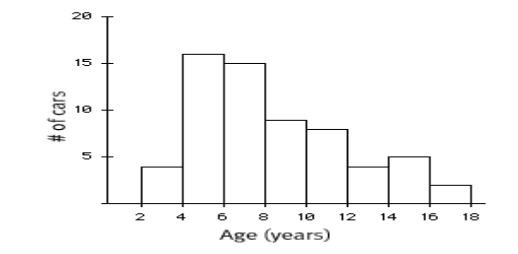
\includegraphics[width=3.17708in,height=\textheight]{images/img24.png}

(a). How many cars are in the first class (between 2 and 4)? In the third class (between 6 and 8)?

(b). Describe the shape of the histogram -- how many modals? Symmetric or skewed (left or right)?

(c). Which measure is more appropriate to use to measure the center? Mean or median?

(d). Which measure is more appropriate to use to measure the spread? Standard deviation or IQR?

\textbf{Exercise 6.} Identify the histogram for the frequency distribution below.

\begin{longtable}[]{@{}ll@{}}
\toprule\noalign{}
Bin & Frequency \\
\midrule\noalign{}
\endhead
\bottomrule\noalign{}
\endlastfoot
{[}2, 7{]} & 3 \\
{[}7, 12{]} & 2 \\
{[}12, 17{]} & 3 \\
{[}17, 22{]} & 6 \\
{[}22, 27{]} & 1 \\
\end{longtable}

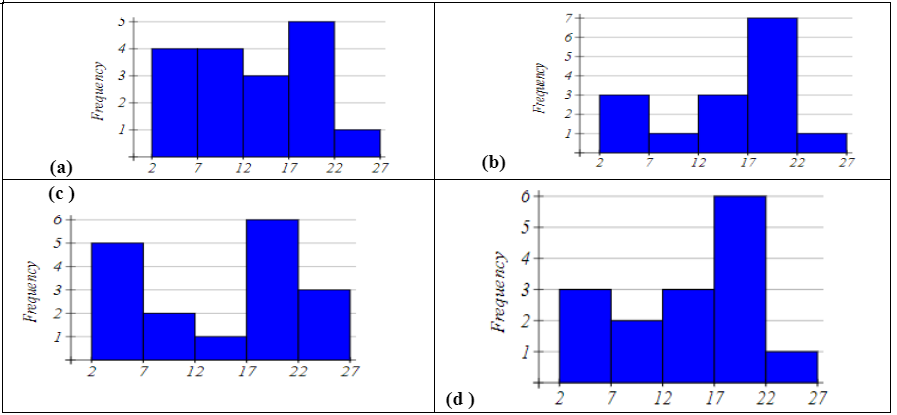
\includegraphics[width=5.63542in,height=\textheight]{images/img26.png}

\textbf{Exercise 7.} Based on the boxplot below:

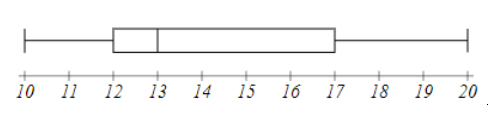
\includegraphics[width=3.08333in,height=\textheight]{images/img27.png}

(a). Write the five number summary.

(b). What percent of data is below 17?

\newpage

\section{Summarizing Categorical Data}\label{summarizing-categorical-data}

\textbf{Objective 3:} By the end of this unit, students will be able to:

\begin{itemize}
\tightlist
\item
  Summarize and describe the distribution of categorical data using contingency tables and various visual displays including bar plots and mosaic plots.
\item
  Explore the association between a numerical variable and a categorical variable using side-by-side box plots.
\end{itemize}

\textbf{Quick Review:}

\begin{enumerate}
\def\labelenumi{\arabic{enumi}.}
\tightlist
\item
  Tables
\end{enumerate}

\begin{itemize}
\tightlist
\item
  Frequency of a category -- the count of that category
\item
  Relative Frequency of a category = \(\frac{\text{Frequency in the category}}{\text{Total number of observations}}\)
\item
  Table (of one variable) -- shows the list of values and the corresponding frequencies (or relative frequencies) of one categorical variable
\item
  Contingency table---presents a summary (of counts or proportions) of two categorical variables bivariate variables
\item
  Computing row and column proportions for contingency table
\end{itemize}

\begin{enumerate}
\def\labelenumi{\arabic{enumi}.}
\setcounter{enumi}{1}
\tightlist
\item
  Bar plots
\end{enumerate}

\begin{itemize}
\tightlist
\item
  Bar plot of one variable -- visualizes the frequencies (or relative frequencies) of one categorical variable
\item
  Bar lots for two categorical variables -- put side by side bar plots
\item
  Stacked bar plot -- stack bars over (using different colors)
\item
  Mosaic plot -- is a special type of standardized stacked bar plots that represents a contingency table. In detailed words, it shows the percentage of one categorical variable (variable 1) for all categories of another variable (variable 2); can use the width of each bar to represent the ratio of variable 2)
\end{itemize}

\begin{enumerate}
\def\labelenumi{\arabic{enumi}.}
\setcounter{enumi}{2}
\item
  Using \textbf{side by side Box plots} for exploring categorical-numerical relationships which provide information about how the distribution of the numeric variable changes across categories.
\item
  R codes (table and bar plot)
\end{enumerate}

\begin{enumerate}
\def\labelenumi{\arabic{enumi})}
\tightlist
\item
  Create a table --- use table()
\end{enumerate}

\texttt{Variable\_Name\ =\ c\ ("category\ 1",\ "Category\ 2",\ …,\ "Category\ n")\ \ \ (Note:\ use\ quotation\ marks\ for\ strings\ –\ categories)}

\texttt{table(Variable\_Name)}

\begin{enumerate}
\def\labelenumi{\arabic{enumi})}
\setcounter{enumi}{1}
\tightlist
\item
  Create Bar plot -- (sample from course notes)
\end{enumerate}

\texttt{\#\ Create\ a\ data\ frame\ with\ the\ Variable\_Name}

\texttt{Variable\_Name\ \textless{}-\ data.frame(}

\texttt{Type\ =\ c("category\ 1",\ "Category\ 2",\ …,\ “Category\ n"),}

\texttt{Frequency\ =\ c(\ f1,f2,\ …,\ fn)\ \ \#\ f1,f2,\ …,fn\ are\ frequencies}

\texttt{\#\ Create\ a\ bar\ plot}

\texttt{barplot(Variable-Name\$Frequency,\ names.arg\ =\ Variable-Name\$Type,}

\texttt{main\ =\ "Frequency\ of\ Variable-Name",}

\texttt{xlab\ =\ "Type\ of\ Variable",\ ylab\ =\ "Frequency",}

\texttt{col\ =\ "blue",\ border\ =\ "black",\ \ \ \ )}

\textbf{Exercise 1.} A survey polled a sample of 350 students for a proposed change of some regulations. The following table summarized the survey response result.

\begin{longtable}[]{@{}lll@{}}
\toprule\noalign{}
Responses & Frequency & Relative Frequency (Round to 3 decimals) \\
\midrule\noalign{}
\endhead
\bottomrule\noalign{}
\endlastfoot
Support & 200 & \\
Neutral & 53 & \\
Oppose & 97 & \\
Total & 350 & \\
\end{longtable}

(a). How many support the proposed change?\\
(b). Fill the last column in the table.\\
(c). What is the percentage of the sampled students who opposed the proposed change?

\textbf{Exercise 2.} The following data is the recorded blood types of 30 volunteers who donated blood at a plasma center.\\
O O A B A A B O AB O\\
B A O A AB O B A B B\\
O O O A A B O B A A

\begin{longtable}[]{@{}lll@{}}
\toprule\noalign{}
Blood Type & Frequency & Relative Frequency \\
\midrule\noalign{}
\endhead
\bottomrule\noalign{}
\endlastfoot
A & & \\
B & & \\
AB & & \\
O & & \\
Total & & \\
\end{longtable}

(a). Summarize the data in a frequency table and calculate the relative frequencies.\\
(b). Draw a histogram for the frequency of the data.

\textbf{Exercise 3.} Four hundred undergraduate students were surveyed about their part time working hours during on semester. The following contingency table summarizes the survey result related to student status and working hours per week.

\begin{longtable}[]{@{}
  >{\raggedright\arraybackslash}p{(\columnwidth - 8\tabcolsep) * \real{0.2527}}
  >{\raggedright\arraybackslash}p{(\columnwidth - 8\tabcolsep) * \real{0.1429}}
  >{\raggedright\arraybackslash}p{(\columnwidth - 8\tabcolsep) * \real{0.2527}}
  >{\raggedright\arraybackslash}p{(\columnwidth - 8\tabcolsep) * \real{0.2747}}
  >{\raggedright\arraybackslash}p{(\columnwidth - 8\tabcolsep) * \real{0.0769}}@{}}
\toprule\noalign{}
\begin{minipage}[b]{\linewidth}\raggedright
\end{minipage} & \begin{minipage}[b]{\linewidth}\raggedright
Not working
\end{minipage} & \begin{minipage}[b]{\linewidth}\raggedright
Work 10 hours or less
\end{minipage} & \begin{minipage}[b]{\linewidth}\raggedright
Work more than 10 hours
\end{minipage} & \begin{minipage}[b]{\linewidth}\raggedright
Total
\end{minipage} \\
\midrule\noalign{}
\endhead
\bottomrule\noalign{}
\endlastfoot
Freshman or Sophomore & 132 & 28 & 20 & 180 \\
Junior or Senior & 120 & 48 & 52 & 220 \\
Total & 252 & 76 & 72 & 400 \\
\end{longtable}

(a). Complete the table for the 2nd row, 3rd row proportions (relative frequencies by class, and overall)\\
(Divide the 2nd row, 3rd row of the table by 220, by 400)

\begin{longtable}[]{@{}
  >{\raggedright\arraybackslash}p{(\columnwidth - 8\tabcolsep) * \real{0.2527}}
  >{\raggedright\arraybackslash}p{(\columnwidth - 8\tabcolsep) * \real{0.1429}}
  >{\raggedright\arraybackslash}p{(\columnwidth - 8\tabcolsep) * \real{0.2527}}
  >{\raggedright\arraybackslash}p{(\columnwidth - 8\tabcolsep) * \real{0.2747}}
  >{\raggedright\arraybackslash}p{(\columnwidth - 8\tabcolsep) * \real{0.0769}}@{}}
\toprule\noalign{}
\begin{minipage}[b]{\linewidth}\raggedright
\end{minipage} & \begin{minipage}[b]{\linewidth}\raggedright
Not working
\end{minipage} & \begin{minipage}[b]{\linewidth}\raggedright
Work 10 hours or less
\end{minipage} & \begin{minipage}[b]{\linewidth}\raggedright
Work more than 10 hours
\end{minipage} & \begin{minipage}[b]{\linewidth}\raggedright
Total
\end{minipage} \\
\midrule\noalign{}
\endhead
\bottomrule\noalign{}
\endlastfoot
Freshman or Sophomore & 0.733 & 0.07 & 0.05 & 1 \\
Junior or Senior & & & & 1 \\
All UG & & & & 1 \\
\end{longtable}

(b). Find the column proportions. Interoperate the meaning the ratios of 2nd, 3rd, and 4th columns

\begin{longtable}[]{@{}
  >{\raggedright\arraybackslash}p{(\columnwidth - 8\tabcolsep) * \real{0.2447}}
  >{\raggedright\arraybackslash}p{(\columnwidth - 8\tabcolsep) * \real{0.1383}}
  >{\raggedright\arraybackslash}p{(\columnwidth - 8\tabcolsep) * \real{0.2447}}
  >{\raggedright\arraybackslash}p{(\columnwidth - 8\tabcolsep) * \real{0.2660}}
  >{\raggedright\arraybackslash}p{(\columnwidth - 8\tabcolsep) * \real{0.1064}}@{}}
\toprule\noalign{}
\begin{minipage}[b]{\linewidth}\raggedright
\end{minipage} & \begin{minipage}[b]{\linewidth}\raggedright
Not working
\end{minipage} & \begin{minipage}[b]{\linewidth}\raggedright
Work 10 hours or less
\end{minipage} & \begin{minipage}[b]{\linewidth}\raggedright
Work more than 10 hours
\end{minipage} & \begin{minipage}[b]{\linewidth}\raggedright
Total
\end{minipage} \\
\midrule\noalign{}
\endhead
\bottomrule\noalign{}
\endlastfoot
Freshman or Sophomore & 132/252= & 28/76= & 20/72= & 180/400= \\
Junior or Senior & 120/252= & 48/76= & 52/72= & 220/400 \\
Total & 252/252= & 76/76= & 72/72= & 400/400 \\
\end{longtable}

(c). Find the overall relative frequencies by dividing all by 400 (grant total) Interoperate the meaning of each.

\begin{longtable}[]{@{}
  >{\raggedright\arraybackslash}p{(\columnwidth - 8\tabcolsep) * \real{0.2447}}
  >{\raggedright\arraybackslash}p{(\columnwidth - 8\tabcolsep) * \real{0.1383}}
  >{\raggedright\arraybackslash}p{(\columnwidth - 8\tabcolsep) * \real{0.2447}}
  >{\raggedright\arraybackslash}p{(\columnwidth - 8\tabcolsep) * \real{0.2660}}
  >{\raggedright\arraybackslash}p{(\columnwidth - 8\tabcolsep) * \real{0.1064}}@{}}
\toprule\noalign{}
\begin{minipage}[b]{\linewidth}\raggedright
\end{minipage} & \begin{minipage}[b]{\linewidth}\raggedright
Not working
\end{minipage} & \begin{minipage}[b]{\linewidth}\raggedright
Work 10 hours or less
\end{minipage} & \begin{minipage}[b]{\linewidth}\raggedright
Work more than 10 hours
\end{minipage} & \begin{minipage}[b]{\linewidth}\raggedright
Total
\end{minipage} \\
\midrule\noalign{}
\endhead
\bottomrule\noalign{}
\endlastfoot
Freshman or Sophomore & 132/400= & 28/400= & 20/400= & 180/400= \\
Junior or Senior & 120/400= & 48/400= & 52/400= & 220/400= \\
Total & 252/400= & 76/400= & 72/400= & 400/400= \\
\end{longtable}

\chapter{Probability Basics Worksheet}\label{probability-basics-worksheet}

\textbf{Objective 1:} By the end of this unit, students will be able to:

\begin{itemize}
\tightlist
\item
  Explain the concept of randomness and how probability quantifies randomness.
\item
  Recognize the basic concepts of sample space, equally likely outcomes, events, unions and intersections.
\item
  Identify when two events are mutually exclusive, independent or complementary.
\item
  Use probability rules to compute the probability of different types of events.
\item
  Distinguish between marginal probability and conditional probability.
\end{itemize}

\section{Quick Review on Probability}\label{quick-review-on-probability}

The starting point in studying probabilities is the concept of an \(\underline{\textbf{experiment or random process}}\), by which we mean some act or observation whose outcome is not known in advance. Simple examples would be

\(\bullet\ \  \text{Rolling a die} \\ \\\)

\(\bullet \ \ \text{Tossing a coin twice} \\ \\\)

\(\bullet \ \ \text{Observing the temperature at GSO at 3:00 pm this afternoon (Fo)} \\\)

Although we cannot predict what we will observe, we can in some cases compile a list of all the outcomes we might observe. This is known as the \(\underline{\textbf{sample space}}\) for the experiment, and is a set in mathematical terms, that is to say a collection of distinct items. Generally for a sample space of n possible outcomes we write \(S = {E1, E2, ... , E_n}\) . For example in the die rolling experiment we have \(\textit{S={1, 2, 3, 4, 5, 6}}\) and in the coin tossing experiment we could list the outcomes as \(\textit{S={TT, TH, HT, HH}}\) It is a little harder to list the sample space for the third experiment, given the current temperature a list of the numbers between 40 and 80 would probably suffice.

We use the outcomes in the sample space for computing probabilities for any event according to the following basic rule:

\[
\textbf{P(A) = the sum of the probabilities of all the outcomes in the event A}
\]

\textbf{Events} in probability are just the same as sets in mathematics, so you should know the principle operations on sets:

\(\bullet\) UNION: A \(\cup\) B (``A or B'') is the set of all outcomes in A or in B or in both

\(\bullet\) INTERSECTION: A \(\cap\) B (``A and B'') is the set of outcomes that are in both A and B

\(\bullet\ \ \text{COMPLEMENT: Ac (“not A”) everything outside of A (but in S)}\)


\includegraphics[width=7.5625in,height=\textheight]{images/img13.png}

It is important to realize that A \(\cup\) B, A \(\cap\) B, and \(A^c\) are all sets, that is to say, they are \textbf{collections of} \(\textit{distinct}\) \textbf{items, and no element may be listed twice.}

For example, with reference to the die rolling experiment, define the event B as ``a number at least as great as 5 comes up'', so B=\{5,6\}. For A=\{2,4,6\} (an even number comes up), we have

\(\bullet\ \  \ A \cup B \text{={2,4,5,6},}\\ \\\)

\(\bullet \ \ \ A\cap B \text{={6},}\\ \\\)

\(\bullet \ \ A^c \text{={1,3,5}}, \\\)

\(\bullet \ \ B^c \text{={1,2,3,4}}\)

Suppose the die is assumed to be fair. This, by definition, means that each side is equally likely to come up when the die is rolled. If we assign a total probability of 1 to the entire sample space, then we should assign a probability of 1/6 to each of the 6 outcomes in the sample space, so

\[
\text{P(1) = P(2) = P(3) = P(4) = P(5) = P(6) = 1/6.}
\]

Thus, we should obtain:

\(P(A) = \frac{1}{6}+\frac{1}{6}+\frac{1}{6}=\frac{3}{6}=\frac{1}{2}\)

\(P(B) = \frac{1}{6}+\frac{1}{6}=\frac{2}{6}=\frac{1}{3}\)

\(P(A \cup B) = \frac{1}{6}+\frac{1}{6}+\frac{1}{6}+\frac{1}{6}=\frac{4}{6}=\frac{2}{3}\)

\(P(A \cap B) = \frac{1}{6}\)

\(P(A^c) = \frac{1}{6}+\frac{1}{6}+\frac{1}{6}=\frac{1}{2}\)

\(P(A^c) = \frac{1}{6}+\frac{1}{6}+\frac{1}{6}+\frac{1}{6}=\frac{2}{3}\)

Some points worth noting:

\(\bullet\) P(A U B) = 4/6 does NOT equal P(A) + P(B) = 5/6 (this is because the two sets have an element, 6, in common).

\(\bullet\) P(Ac) = 1 - P(A) and P(Bc) = 1 -- P(B).

\(\bullet\) Also note that in cases where all the outcomes in the sample space are equally likely, the rule about adding the probabilities for all of the outcomes in the event simplifies to counting the number of outcomes in the event and dividing by the number out outcomes in the sample space. So, for the events A and B above, P(A) = 3/6 = 1⁄2, and P(B) = 2/6 = 1/3.

\(\bullet\) Generally, if A contains m outcomes, and the sample space has n equally likely outcomes (so the probability for each outcome is 1/n), then P(A) = m/n.

At this stage, let us write down some \textbf{general rules or AXIOMS for probability.} The events A, B below are now general events in a sample space, not the specific ones described above.

\begin{enumerate}
\def\labelenumi{\arabic{enumi})}
\tightlist
\item
  For any sample space, P(S) = 1
\item
  For any event A, 0 \(\le\) P(A) \(le\) 1
\item
  General addition rule: If A and B are any two events, disjoint or not, then the probability that at least one of them will occur is
\end{enumerate}

\[
\text{P (A or B) = P (A) + P (B) - P (A and B) }
\]

where P(A and B) is the probability that both events occur. Here, A or B occurs means A, B, or both A and B occur.

4)Addition rule for disjoint events: For any events A, B which have no common outcomes,

\[
\text{P(A U B) = P(A) + P(B)}
\]

Events which have no outcomes in common are often referred to as \textbf{mutually exclusive} (or \(\textit{disjoint}\)). If two events A, B are mutually exclusive, we write P(A \(\cap\) B) = \(\emptyset\) , where \(\emptyset\) is referred to as the \(\textit{empty set}\). It is sort of equivalent to the number zero in arithmetic.

Note that using the first and third rules, we have \(1 = P(S) = P(A \cup A^c) = P(A) + P(A^c)\) ) , so we have a general rule that for any set \(A, \ P(A^c) = 1 – P(A)\). This is often called the \textbf{law of complements}.

\textbf{Exercise 1.} A set of 11 cards is numbered 1 through 11. A card is picked at random and the following events defined: A - the number on card is odd: B - the number on the card is 5 or higher. Find

\begin{enumerate}
\def\labelenumi{\alph{enumi})}
\item
  P(A) =
\item
  P(B) =
\item
  P(A and B) =
\item
  P(A or B) =
\end{enumerate}

\textbf{Exercise 2.} (Sample space where the outcomes are NOT equally likely): Professor Donald Fraser of the University of Toronto constructed a (purposely) uneven die. On inspection it was clear that the sides would not have equal probability. He rolled it 12,800 times, and came up with the following empirical probabilities (based on relative frequency):

\begin{longtable}[]{@{}lllllll@{}}
\toprule\noalign{}
Side & 1 & 2 & 3 & 4 & 5 & 6 \\
\midrule\noalign{}
\endhead
\bottomrule\noalign{}
\endlastfoot
Probability & 0.186 & 0.179 & 0.207 & 0.137 & 0.149 & 0.142 \\
\end{longtable}

For the events A (even number) and B (at least 5) compute:

\begin{enumerate}
\def\labelenumi{\alph{enumi})}
\item
  \(\text{P(A) =}\)
\item
  \(\text{P(B) =}\)
\item
  \(P(A \cup B)=\)
\item
  \(P(A\cap B) =\)
\item
  \(P(A^c) =\)
\item
  \(P(B^c) =\)
\end{enumerate}

\textbf{Exercise 3.} A group of 1000 students is classified by gender \(G_1\) (male) or \(G_2\) (female), and by year, \(\textbf{Y}_1\) (freshman), \(\textbf{Y}_2\) (sophomore), \(\textbf{Y}_3\) (junior), or \(\textbf{Y}_4\) (senior). This results in the following table:

\begin{longtable}[]{@{}
  >{\raggedright\arraybackslash}p{(\columnwidth - 10\tabcolsep) * \real{0.1667}}
  >{\raggedright\arraybackslash}p{(\columnwidth - 10\tabcolsep) * \real{0.1667}}
  >{\raggedright\arraybackslash}p{(\columnwidth - 10\tabcolsep) * \real{0.1667}}
  >{\raggedright\arraybackslash}p{(\columnwidth - 10\tabcolsep) * \real{0.1667}}
  >{\raggedright\arraybackslash}p{(\columnwidth - 10\tabcolsep) * \real{0.1667}}
  >{\raggedright\arraybackslash}p{(\columnwidth - 10\tabcolsep) * \real{0.1667}}@{}}
\toprule\noalign{}
\begin{minipage}[b]{\linewidth}\raggedright
\end{minipage} & \begin{minipage}[b]{\linewidth}\raggedright
Freshman (\(Y_1\))
\end{minipage} & \begin{minipage}[b]{\linewidth}\raggedright
Sophomore (\(Y_2\))
\end{minipage} & \begin{minipage}[b]{\linewidth}\raggedright
Junior (\(Y_3\))
\end{minipage} & \begin{minipage}[b]{\linewidth}\raggedright
Senior (\(Y_4\))
\end{minipage} & \begin{minipage}[b]{\linewidth}\raggedright
Total
\end{minipage} \\
\midrule\noalign{}
\endhead
\bottomrule\noalign{}
\endlastfoot
Male (\(G_1\)) & 140 & 120 & 110 & 70 & 440 \\
Female (\(G_2\)) & 160 & 130 & 140 & 130 & 560 \\
Total & 300 & 250 & 250 & 200 & 1000 \\
\end{longtable}

If a student is randomly selected, find the probability that the student:

\begin{enumerate}
\def\labelenumi{\alph{enumi})}
\item
  Is a junior, P(\(Y_3\)) =
\item
  Is a female freshman, P(\(G_2\) and \(Y_1\)) =
\item
  Is a male or a junior, P(\(G_1\) or \(Y_3\)) =
\end{enumerate}

d)Is not a freshman, P(not \(Y_1\)) =

\begin{enumerate}
\def\labelenumi{\alph{enumi})}
\setcounter{enumi}{4}
\tightlist
\item
  Is not a male and is not a junior, P(not \(G_1\) and not \(Y_3\)) =
\end{enumerate}

\textbf{Exercise 4.} Here is the ``Craps Game'' sample space, where a red and a green die are rolled. Each outcome (i,j) represents the red die coming up i and the green die coming up j.

\begin{longtable}[]{@{}lllllll@{}}
\toprule\noalign{}
& j=1 & j=2 & j=3 & j=4 & j=5 & j=6 \\
\midrule\noalign{}
\endhead
\bottomrule\noalign{}
\endlastfoot
\textbf{i=1} & (1,1) & (1,2) & (1,3) & (1,4) & (1,5) & (1,6) \\
\textbf{i=2} & (2,1) & (2,2) & (2,3) & (2,4) & (2,5) & (2,6) \\
\textbf{i=3} & (3,1) & (3,2) & (3,3) & (3,4) & (3,5) & (3,6) \\
\textbf{i=4} & (4,1) & (4,2) & (4,3) & (4,4) & (4,5) & (4,6) \\
\textbf{i=5} & (5,1) & (5,2) & (5,3) & (5,4) & (5,5) & (5,6) \\
\textbf{i=6} & (6,1) & (6,2) & (6,3) & (6,4) & (6,5) & (6,6) \\
\end{longtable}

There are n=36 outcomes, and for fair dice it is reasonable to assume they are equally likely.\textbf{Find the probability of each of the following events. Identify which pairs of events are disjoint.}

\begin{enumerate}
\def\labelenumi{(\alph{enumi})}
\item
  A ``sum is 7'':

  P(A) =
\item
  B ``sum is 11'':

  P(B) =
\item
  C ``sum is 6'':

  P(C) =
\item
  D ``both dice show same number'':

  P(D) =
\item
  E ``both dice odd'':

  P(E) =
\item
  F ``both dice even'':

  P(F) =
\end{enumerate}

\textbf{Exercise 5. True or False}

\begin{enumerate}
\def\labelenumi{\alph{enumi})}
\item
  If A and B are mutually exclusive (disjoint) events, then P(A and B) = 0.
\item
  For any event A, P(A) + P(\(A^c\)) = 1.
\end{enumerate}

\textbf{Solution}

Question 1:

Since, A = \{1,3,5,7,9,11\}, B= \{5,6,7,8,9,10,11\}, (A and B) = \{5,7,9,11\} and (A or B)=\{1,3,5,6,7,8,9,10,11\}

\begin{enumerate}
\def\labelenumi{\alph{enumi})}
\item
  \(\text{P(A)}=\frac{6}{11}\)
\item
  \(\text{P(B)}=\frac{7}{11}\)
\item
  \(\text{P(A and B)}=\frac{4}{11}\)
\item
  \(\text{P(A or B)=P(A)+P(B)-P(A and B)}\\=\frac{6}{11}+\frac{7}{11}-\frac{4}{11}=\frac{9}{11}\)
\end{enumerate}

Question 2:

A = \{2,4,6\}, B= \{5,6\}, (A\(\cup\)B) = \{2,4,5,6\} and (A \(\cap\) B)=\{6\}

\begin{enumerate}
\def\labelenumi{\alph{enumi})}
\item
  \(\text{P(A)=P(2)+P(4)+P(6)=}0.179+0.137+0.142=0.458\)
\item
  \(\text{P(B)=P(5)+P(6)}=0.149+0.142=0.291\)
\item
  \(\text{P(A U B)}=\text{P(2)+P(4)+P(5)+P(6)}=0.179+0.137+0.149+0.142 \\=0.607\)
\item
  P(A\(\cap\)B)=P(6)=0.142
\item
  P(\(A^c\))= 1 - P(A) = 1 - 0.458 = 0.542
\item
  P(\(B^c\))= 1 - P(B) = 1 - 0.291 = 0.709
\end{enumerate}

Question 3:

The probability that the student :

\begin{enumerate}
\def\labelenumi{\alph{enumi})}
\item
  Is a junior, P(\(Y_3\)) = \(\frac{250}{1000}=0.25\)
\item
  Is a female freshman, P(\(G_2\) and \(Y_1\))= \(\frac{160}{1000}=0.16\)
\item
  Is a male or a junior, P(\(G_1\) or \(Y_3\))= \(\frac{440+140}{1000}=\frac{580}{1000}=0.580\)

  or P(\(G_1\))+ P(\(Y_3\)) - P(\(G_1\) and \(Y_3\)) = \(\frac{440}{1000}+\frac{250}{1000}-\frac{110}{1000}\)
\item
  Is not a freshman, P(not \(Y_1\))= 1 - P(\(Y_1\)) = 1 - (\(\frac{300}{1000}\)) =1 - 0.3 = 0.70
\item
  Is not a male and is not a junior, P (not \(G_1\) and not \(Y_3\)) = \(\frac{150+130+130}{1000}\) = \(\frac{420}{1000}=0.420\)
\end{enumerate}

Question 4:

Note: For this question, also ask them to identify which pair of event are disjoint.

\begin{enumerate}
\def\labelenumi{\alph{enumi})}
\tightlist
\item
  A ``sum is 7'' : \{(1,6),(6,1), (2,5), (5,2), (3,4), (4,3)\}
\end{enumerate}

P(A) = \(\frac{6}{36}=\frac{1}{6}\)

\begin{enumerate}
\def\labelenumi{\alph{enumi})}
\setcounter{enumi}{1}
\tightlist
\item
  B ``sum is 11'': \{(5,6),(6,5)\}
\end{enumerate}

P(A) = \(\frac{2}{36}=\frac{1}{18}\)

\begin{enumerate}
\def\labelenumi{\alph{enumi})}
\setcounter{enumi}{2}
\tightlist
\item
  C ``sum is 6'': \{(1,5), (5,1), (2,4), (4,2), (3,3)\}
\end{enumerate}

P(C) = \(\frac{5}{36}\)

\begin{enumerate}
\def\labelenumi{\alph{enumi})}
\setcounter{enumi}{3}
\tightlist
\item
  D ``both dice show small number'': \{(1,1), (2,2), (3,3), (4,4), (5,5),(6,6)\}
\end{enumerate}

P(D) = \(\frac{6}{36}=\frac{1}{6}\)

\begin{enumerate}
\def\labelenumi{\alph{enumi})}
\setcounter{enumi}{4}
\tightlist
\item
  E ``both dice odd'': \{(1,1), (1,3), (1,5), (3,1), (3,3),(3,5),(5,1),(5,3),(5,5)\}
\end{enumerate}

P(E) = \(\frac{9}{36}=\frac{1}{4}\)

\begin{enumerate}
\def\labelenumi{\alph{enumi})}
\setcounter{enumi}{5}
\tightlist
\item
  F ``both dice even'': \{(2,2), (2,4), (2,6), (4,2), (4,4),(4,6),(6,2),(6,4),(6,6)\}
\end{enumerate}

P(F) = \(\frac{9}{36}=\frac{1}{4}\)

Question 5:

\begin{enumerate}
\def\labelenumi{\alph{enumi})}
\item
  If A and B are mutually exclusive (disjoint) events, then P(A and B) = 0.

  Ans : TRUE

  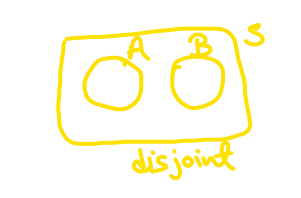
\includegraphics[width=2.375in,height=\textheight]{images/img17.png}
\item
  For any event A, P(A) + P(\(A^c\)) = 1.

  Ans : TRUE

  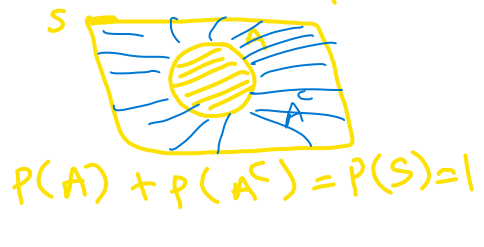
\includegraphics[width=3.0625in,height=\textheight]{images/img18.png}
\end{enumerate}

\section{Discrete Random Variables}\label{discrete-random-variables}

\textbf{Objective 2:} By the end of this unit, students will be able to:

\begin{itemize}
\tightlist
\item
  Use probability rules to compute the probability of different types of events.
\item
  Distinguish between marginal probability and conditional probability.
\item
  Apply the multiplication rule to compute probabilities when sampling with/without replacement from finite populations.
\item
  Define random variables.
\item
  Compute expectation and variance of discrete random variables.
\end{itemize}

\textbf{Exercise: Profit from crop yield under different weather conditions (X).}

\textbf{Exercises}

\begin{enumerate}
\def\labelenumi{\arabic{enumi}.}
\tightlist
\item
  Determine the missing probability in the following distribution.
\end{enumerate}

\begin{longtable}[]{@{}lll@{}}
\toprule\noalign{}
Weather & Profit (\$) & Probability \\
\midrule\noalign{}
\endhead
\bottomrule\noalign{}
\endlastfoot
Dry & 200,000 & 0.30 \\
Light Rain & 300,000 & 0.50 \\
Storm & 150,000 & ? \\
\end{longtable}

\begin{enumerate}
\def\labelenumi{\arabic{enumi}.}
\setcounter{enumi}{1}
\tightlist
\item
  Find the expected profit from this crop, \(\mu\).
\end{enumerate}

\begin{longtable}[]{@{}lll@{}}
\toprule\noalign{}
\(x_i\) & \(P(x_i)\) & \(x_i P(x_i)\) \\
\midrule\noalign{}
\endhead
\bottomrule\noalign{}
\endlastfoot
200,000 & 0.30 & \(200,000 \times 0.30\) \\
300,000 & 0.50 & \(300,000 \times 0.50\) \\
150,000 & ? & \(150,000 \times ?\) \\
\end{longtable}

\begin{enumerate}
\def\labelenumi{\arabic{enumi}.}
\setcounter{enumi}{2}
\tightlist
\item
  Find the variance, \(\sigma^2\) and the standard deviation, \(\sigma\).
\end{enumerate}

\begin{longtable}[]{@{}
  >{\raggedright\arraybackslash}p{(\columnwidth - 10\tabcolsep) * \real{0.1098}}
  >{\raggedright\arraybackslash}p{(\columnwidth - 10\tabcolsep) * \real{0.1220}}
  >{\raggedright\arraybackslash}p{(\columnwidth - 10\tabcolsep) * \real{0.0854}}
  >{\raggedright\arraybackslash}p{(\columnwidth - 10\tabcolsep) * \real{0.1829}}
  >{\raggedright\arraybackslash}p{(\columnwidth - 10\tabcolsep) * \real{0.2073}}
  >{\raggedright\arraybackslash}p{(\columnwidth - 10\tabcolsep) * \real{0.2927}}@{}}
\toprule\noalign{}
\begin{minipage}[b]{\linewidth}\raggedright
\(x_i\)
\end{minipage} & \begin{minipage}[b]{\linewidth}\raggedright
\(P(x_i)\)
\end{minipage} & \begin{minipage}[b]{\linewidth}\raggedright
\(\mu\)
\end{minipage} & \begin{minipage}[b]{\linewidth}\raggedright
\((x_i - \mu)\)
\end{minipage} & \begin{minipage}[b]{\linewidth}\raggedright
\((x_i - \mu)^2\)
\end{minipage} & \begin{minipage}[b]{\linewidth}\raggedright
\((x_i - \mu)^2 P(x_i)\)
\end{minipage} \\
\midrule\noalign{}
\endhead
\bottomrule\noalign{}
\endlastfoot
200,000 & 0.30 & & & & \\
300,000 & 0.50 & & & & \\
150,000 & ? & & & & \\
\end{longtable}

The standard deviation is \(\sigma\) = \_\_\_\_\_\_\_\_\_\_\_\_\_\_\_\_

\begin{enumerate}
\def\labelenumi{\arabic{enumi}.}
\setcounter{enumi}{3}
\tightlist
\item
  Interpret the value of the expected profit, \(\mu\).
\end{enumerate}

\textbf{Example/Exercise: 40\% of all voters support Proposition A. If a random sample of 10 voters is polled. Find the following probabilities.}

\textbf{Formula for the probability of exactly \(x\) successes from \(n\) trials}

\[
p(x) = \binom{n}{x} p^x q^{n-x} = \frac{n!}{(n-x)!x!} p^x q^{n-x}; \quad \text{where } x = 0, 1, 2, \ldots, n
\]

and

\[
n! = n(n-1)(n-2) \cdots (3)(2)(1)
\]

\begin{enumerate}
\def\labelenumi{\arabic{enumi}.}
\tightlist
\item
  What is the probability that exactly five of them support the proposition?
\end{enumerate}

Using the binomial probability formula:
\[
   P(X = k) = \binom{n}{k} p^k (1-p)^{n-k}
   \]
where \(n = 10\), \(k = 5\), and \(p = 0.4\).

\begin{enumerate}
\def\labelenumi{\arabic{enumi}.}
\setcounter{enumi}{1}
\item
  What is the probability that five or six of them support the proposition?
\item
  What is the probability that at least three of them support the proposition?
\end{enumerate}

\textbf{Exercise:} the manufacturer of the ColorSmart-5000 television set claims that 95\% of
its sets last at least five years without requiring a single repair. Suppose that we contact 8 randomly selected ColorSmart-5000 purchasers five years after they purchased their sets
and ask each purchaser: Have you needed any repair for your ColorSmart-5000 TV set
during the first 5 years after purchasing the set?

\begin{enumerate}
\def\labelenumi{\arabic{enumi}.}
\item
  Find the probability that exactly 7 customers needed at least one repair during the first 5 years.
\item
  Find the probability that at least 7 purchasers needed at least one repair during the first 5 years.
\end{enumerate}

\textbf{Solution}

Exercise: Profit from crop yield under different weather condi-tions (X).
1. Determine the missing probability in the following distribution.

\begin{longtable}[]{@{}lll@{}}
\toprule\noalign{}
\textbf{Weather} & \textbf{Profit (\$)} & \textbf{Probability} \\
\midrule\noalign{}
\endhead
\bottomrule\noalign{}
\endlastfoot
Dry & 200,000 & 0.30 \\
Light Rain & 300,000 & 0.50 \\
Storm & 150,000 & ? \\
\end{longtable}

\begin{enumerate}
\def\labelenumi{\arabic{enumi}.}
\setcounter{enumi}{1}
\tightlist
\item
  Find the expected profit from this crop, \(\mu\).
\end{enumerate}

\[
\begin{aligned}
\mu &= \sum{x_i}P(x_i) \\
    &= \$200k \cdot 0.3 + \$300k \cdot 0.5 + \$150k \cdot 0.2 \\
    &= \$60k + \$150k + \$30k = \$240k
\end{aligned}
\]

\begin{enumerate}
\def\labelenumi{\arabic{enumi}.}
\setcounter{enumi}{2}
\tightlist
\item
  Find the variance, \(\sigma^2\) and the standard deviation, \(\sigma\).
\end{enumerate}

\[
\begin{aligned}
\sigma^2 &= \sum(x_i-\mu)^2P(x_i) \\
&= (\$200k-\$240k)^2 \ . 0.3 + (\$300k-\$240k)^2 \ . 0.5 + (\$150k-\$240)^2 . 0.2 \\
&= \$^2 3,900, 000, 000 \\
\end{aligned}
\]

The standard deviation is \(\sigma = \sqrt{\$^2 3,900,000,000}\) = \$62,450

\begin{enumerate}
\def\labelenumi{\arabic{enumi}.}
\setcounter{enumi}{3}
\tightlist
\item
  Interpret the value of the expected profit, \(\mu\).
\end{enumerate}

The expected profit represents the long-run average, the expected profit on average in the future.

\textbf{Example/Exercise: 40\% of all voters support Proposition A. If a random sample of 10 voters is polled. Find the following probabilities.}

\begin{enumerate}
\def\labelenumi{\arabic{enumi}.}
\tightlist
\item
  What is the probability that exactly five of them support the proposition?
\end{enumerate}

\[
\begin{aligned}
P(X=5)&=\frac{10!}{(10-5)!5!}(0.40)^5(0.60)^{10-5} \\
&=\frac{10!}{5!5!}(0.40)^5(0.60)^5 \\
&=(252)(0.01024)(0.07776) \\
&=0.2007
\end{aligned}
\]

\begin{enumerate}
\def\labelenumi{\arabic{enumi}.}
\setcounter{enumi}{1}
\tightlist
\item
  What is the probability that five or six of them support the proposition?
\end{enumerate}

\[
\begin{aligned}
P(X=5)+P(X=6)&=0.2007+\frac{10!}{(10-6)!6!}(0.40)^6(0.60)^{10-6} \\
&=0.2007+\frac{10!}{4!6!}(0.40)^6(0.60)^4 \\
&=0.2007+(210)(0.004096)(0.1296) \\
&=0.2007+0.1115 \\
&=0.312
\end{aligned}
\]

\begin{enumerate}
\def\labelenumi{\arabic{enumi}.}
\setcounter{enumi}{2}
\tightlist
\item
  What is the probability that at least three of them support the proposition?
\end{enumerate}

\[
\begin{aligned}
P(x \ge 3) &= P(X=3)+P(X=4)+P(X=5)+P(X=6)+...+P(X=10) \\
&=1-[P(X=0)+P(X=1)+P(X=2)] \\
&=1-[\frac{10!}{0!10!}(0.40)^0(0.60)^{10}+\frac{10!}{1!9!}(0.40)^1(0.60)^9+\frac{10!}{2!8!}(0.40)^2(0.60)^8] \\
&=1-[(1)(1)(0.0060)+(10)(0.40)(0.0101)+(45)(0.16)(0.0168)] \\
&=1-[0.0060+0.0403+0.1209] \\
&=1-0.1672 = 0.8328
\end{aligned}
\]

\textbf{Exercise:} the manufacturer of the ColorSmart-5000 television set claims that 95\% of
its sets last at least five years without requiring a single repair. Suppose that we contact 8 randomly selected ColorSmart-5000 purchasers five years after they purchased their sets and ask each purchaser: Have you needed any repair for your ColorSmart-5000 TV set during the first 5 years after purchasing the set?

\begin{enumerate}
\def\labelenumi{\arabic{enumi}.}
\tightlist
\item
  Find the probability that exactly 7 customers needed at least one repair during the first 5years.
\end{enumerate}

\[
\begin{aligned}
P(X=7)&=\frac{8!}{(8-7)!7!}(0.05)^7(0.95)^{8-7} \\
&=\frac{8!}{1!7!}(0.05)^7(0.95)^1 \\
&=0.0000000059375
\end{aligned}
\]

\begin{enumerate}
\def\labelenumi{\arabic{enumi}.}
\setcounter{enumi}{1}
\tightlist
\item
  Find the probability that at least 7 purchasers needed at least one repair during the first 5years.
\end{enumerate}

\[
\begin{aligned}
P(X=7)&=P(X=7)+P(X=8)\\
&=0.0000000059375+\frac{8!}{(8-8)!8!}(0.05)^8(0.95)^{8-8} \\
&=0.0000000059375+0.0000000000390625 \\
&=0.0000000059765625
\end{aligned}
\]

\section{Binomial Distribution}\label{binomial-distribution}

\textbf{Objective 3:} By the end of this unit, students will be able to:

\begin{itemize}
\tightlist
\item
  Identify when the conditions apply for the Binomial distribution to be used.
\item
  Apply the Binomial distribution to model counts resulting from binary trials.
\end{itemize}

\textbf{Binomial Distribution Condition}

Conditions to be satisfied for a Binomial Variable Distribution with a fixed number of trials \(n\):

\begin{itemize}
\tightlist
\item
  The trials are independent
\item
  Each trial has two possible outcomes classified as success or failure
\item
  The probability of a success \(p\) is the same for each trial
\end{itemize}

\textbf{Probability Mean and Standard Deviation}

For a binomial random variable \(X\) with \(n\) trials and the probability of a single trial being a success \(p\), the probability of observing exactly \(k\) successes is

\[
P(X = k) = \binom{n}{k} p^k (1-p)^{n-k} = \frac{n!}{k!(n-k)!} p^k (1-p)^{n-k} \quad (k = 0, 1, \ldots, n)
\]

Where: - \(n! = 1 \times 2 \times \cdots \times n\) - \(0! = 1\) - \(\binom{n}{k} = \frac{n!}{k!(n-k)!}\) (read as ``n choose k'', also called the combination coefficient)

Mean: \(\mu = np\)

Standard deviation: \(\sigma = \sqrt{np(1-p)}\)

Observations that are more than 2 standard deviations away from the mean are considered unusual:

Unusual if outside of \(\mu - 2\sigma\) and \(\mu + 2\sigma\)

\textbf{Shape of Binomial Distribution}

\begin{itemize}
\tightlist
\item
  For \(p < 0.5\): skew to the left
\item
  For \(p > 0.5\): skew to the right
\item
  For \(p = 0.5\): symmetric (centered at \(\mu\))
\item
  For large \(n\), if \(np \geq 10\) and \(n(1-p) \geq 10\), the graph is approximately bell-shaped.
\end{itemize}

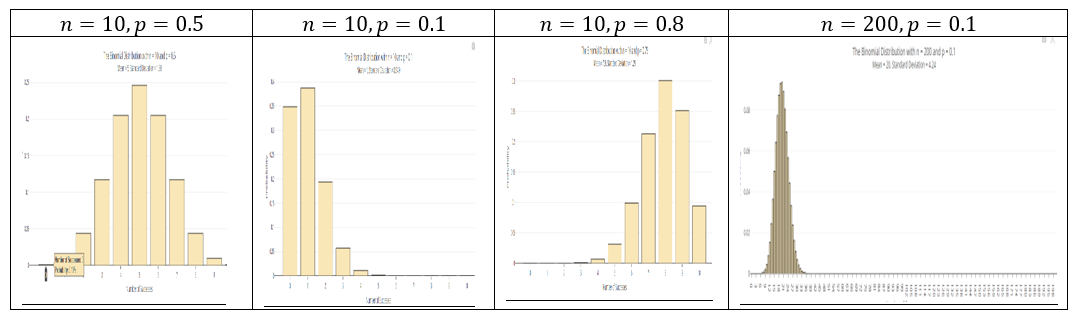
\includegraphics[width=5.72917in,height=\textheight]{images/img41.png}

(Generated using online app \url{https://istats.shinyapps.io/BinomialDist/})

\textbf{Using R}

\begin{itemize}
\item
  For \(P(X = k)\): \texttt{dbinom(k,\ n,\ p)}
\item
  For \(P(X \leq k) = P(X < k+1) = P(X = 0) + P(X = 1) + \cdots + P(X = k)\): \texttt{pbinom(k,\ n,\ p,\ lower.tail\ =\ TRUE)} (the \texttt{lower.tail\ =\ TRUE} can be omitted)
\item
  For \(P(X > k) = P(X \geq k+1) = 1 - P(X \leq k) = P(X = k+1) + \cdots + P(X = n)\): \texttt{pbinom(k,\ n,\ p,\ lower.tail\ =\ FALSE)}
\item
  For \(n!\): \texttt{factorial(n)}
\item
  For \(\binom{n}{k}\): \texttt{choose(n,\ k)}
\end{itemize}

\textbf{Using Calculator}

\begin{enumerate}
\def\labelenumi{\arabic{enumi}.}
\tightlist
\item
  For \(P(X = x)\):

  \begin{itemize}
  \tightlist
  \item
    \texttt{2ND} → \texttt{VARS} (\texttt{DISTR}) → use arrow to select \texttt{binompdf} (enter \(n\), \(p\), \(x\)) then \texttt{enter}
  \end{itemize}
\item
  For \(P(X \leq x)\):

  \begin{itemize}
  \tightlist
  \item
    \texttt{2ND} → \texttt{VARS} (\texttt{DISTR}) → use arrow to select \texttt{binomcdf} (enter \(n\), \(p\), \(x\)) then \texttt{enter}
  \end{itemize}
\item
  For \(n!\):

  \begin{itemize}
  \tightlist
  \item
    Example: \(7!\)
  \item
    Enter 7 then press \texttt{Math} key; use (right) arrow key to select \texttt{PROB} then use (down) arrow key to select \texttt{!} (press enter it then shows \texttt{7!}); press the \texttt{enter} key again (to get answer 5040)
  \end{itemize}
\item
  For \(\binom{n}{k}\):

  \begin{itemize}
  \tightlist
  \item
    Example: \(\binom{9}{2}\)
  \item
    Enter 9 then \texttt{MATH} → arrow to \texttt{PROB} → choose \texttt{nCr} then enter 2 then \texttt{enter} to get the result (answer is 36)
  \end{itemize}
\end{enumerate}

\textbf{Exercise 1}. How many ways can we choose 2 students from a group of 6?

\textbf{Exercise 2} (Combination Formula)

Survey four randomly selected students and record the outcomes as ``I'' (in state) or ``O'' (out state). Fill the table below.

\begin{longtable}[]{@{}
  >{\raggedright\arraybackslash}p{(\columnwidth - 6\tabcolsep) * \real{0.2055}}
  >{\raggedright\arraybackslash}p{(\columnwidth - 6\tabcolsep) * \real{0.2055}}
  >{\raggedright\arraybackslash}p{(\columnwidth - 6\tabcolsep) * \real{0.2055}}
  >{\raggedright\arraybackslash}p{(\columnwidth - 6\tabcolsep) * \real{0.3836}}@{}}
\toprule\noalign{}
\begin{minipage}[b]{\linewidth}\raggedright
\# of ``I''
\end{minipage} & \begin{minipage}[b]{\linewidth}\raggedright
Outcomes (list all)
\end{minipage} & \begin{minipage}[b]{\linewidth}\raggedright
\# of outcomes
\end{minipage} & \begin{minipage}[b]{\linewidth}\raggedright
\(\binom{4}{k} = \frac{4!}{k!(4-k)!}\)
\end{minipage} \\
\midrule\noalign{}
\endhead
\bottomrule\noalign{}
\endlastfoot
\(k = 0\) & & & \\
\(k = 1\) & & & \\
\(k = 2\) & & & \\
\(k = 3\) & & & \\
\(k = 4\) & & & \\
\end{longtable}

\textbf{Exercise 3} Find the probability of success of the Bernoulli trial with \(n\) trials, success probability \(p\), and the success \(k\):

\begin{itemize}
\tightlist
\item
  \(n = 3\), \(k = 2\), \(p = 0.35\)
\item
  \(n = 5\), \(k = 3\), \(p = 0.2\)
\end{itemize}

\textbf{Exercise 4}

For a binomial distribution with \(n = 4\), \(p = 0.7\). (As in exercise 1, assume that 70\% are in-state students.)

(a). Write the formula for computing the probability of getting exactly \(k\) successes.

(b). Fill the following distribution table. (Round to 4 decimals) (you may use R calculator)

\begin{longtable}[]{@{}lll@{}}
\toprule\noalign{}
\(X\) & \(P(X = k)\) & \(P(X \leq k)\) \\
\midrule\noalign{}
\endhead
\bottomrule\noalign{}
\endlastfoot
0 & & \\
1 & & \\
2 & & \\
3 & & \\
4 & & 1 \\
Total & 1 & \\
\end{longtable}

(c). What is the expected value?\\
(d). What is the standard deviation?

\textbf{Exercise 5}

About 75\% of dog owners buy holiday presents for their dogs. Suppose twenty dog owners are randomly selected, find the probability of:

(a). Exactly three buy their dog holiday presents

(b). Exactly seventeen do not buy their dog holiday presents

(c). Three or more buy their dog holiday presents

(d). At most four buy their dog holiday presents

(e). Minimum of 11 and maximum of 17 dog owners buy their dog holiday presents

(f). Find the expected number of dog owners in this sample, who buy their dog holiday presents.

(g). Is it unusual if 16 out of 20 randomly selected dog owners buy their dog holiday presents? Why?

(h). Is it unusual if 10 out of 20 randomly selected dog owners buy their dog holiday presents? Why?

\(\underline{\textbf{Review on Binomial Distribution}}\)

\textbf{Conditions}to be satisfied for a Binomial Variable Distribution:

\(\bullet \ \ \text{The number of trials,is a fixed positive integer}\)

\(\bullet \ \ \text{The trials are independent}\)

\(\bullet \ \ \text{Each trail has two possible outcomes, classified as success or failure}\)

\(\bullet \ \ \text{The probability of a success, p, is the same for each trial}\)

Binomial Distribution

For a binomial random variable with trials and the probability of a single trial being a success the probability of observing exactly successes is

\(P(X =k) = \binom nkp^k(1-p)^{n-k}=\frac{n!}{k! (n-k)!}p^k(1-p)^{n-k} \text{  k= 0,1, ..., n}\)

Accumulative Probability

(at most k success) \(P(X\le k)=P(X <k+1)=\sum_{i=0}^{k}P(X=i)\)

(at least k success) \(P(X\ge k)=P(X>k-1)=1-P(X\le k-1)=\sum_{i=k}^n P(X=i)\)

\(\underline{\textbf{Factorial and Combination Coefficient}}\)

n! = \(1 \times 2 \times ... \times n\) 0! = 1

\(\binom nk = \frac{n!}{k!(n-k)!}\) (\(\binom nk\) is read as ``n choose k'')

\textbf{Solution}

\textbf{Exercise 1. How many ways can we choose 2 students from a group of 6?}

\begin{Shaded}
\begin{Highlighting}[]
\FunctionTok{choose}\NormalTok{(}\DecValTok{6}\NormalTok{,}\DecValTok{2}\NormalTok{)}
\end{Highlighting}
\end{Shaded}

\begin{verbatim}
## [1] 15
\end{verbatim}

\textbf{Exercise 4.} For a binomial distribution with n=4,p=0.2.

\textbf{a) Write the formula for computing the probability of getting exactly k successes.}

\(P(X =k) = \binom nkp^k(1-p)^{n-k}=\frac{n!}{k! (n-k)!}p^k(1-p)^{n-k} \text{  k= 0,1, ..., n}\)

In R you use dbinom(k,n,p)

\textbf{b) Fill the following distribution table. (Round to 4 decimals) (you may use R calculator)}

\begin{Shaded}
\begin{Highlighting}[]
\DocumentationTok{\#\# For P(X=x)}
\FunctionTok{dbinom}\NormalTok{(}\FunctionTok{c}\NormalTok{(}\DecValTok{0}\NormalTok{,}\DecValTok{1}\NormalTok{,}\DecValTok{2}\NormalTok{,}\DecValTok{3}\NormalTok{,}\DecValTok{4}\NormalTok{), }\DecValTok{4}\NormalTok{, }\FloatTok{0.2}\NormalTok{)}
\end{Highlighting}
\end{Shaded}

\begin{verbatim}
## [1] 0.4096 0.4096 0.1536 0.0256 0.0016
\end{verbatim}

\begin{Shaded}
\begin{Highlighting}[]
\DocumentationTok{\#\# P(X \textless{}= x)}
\FunctionTok{pbinom}\NormalTok{(}\FunctionTok{c}\NormalTok{(}\DecValTok{0}\NormalTok{,}\DecValTok{1}\NormalTok{,}\DecValTok{2}\NormalTok{,}\DecValTok{3}\NormalTok{,}\DecValTok{4}\NormalTok{), }\DecValTok{4}\NormalTok{, }\FloatTok{0.2}\NormalTok{)}
\end{Highlighting}
\end{Shaded}

\begin{verbatim}
## [1] 0.4096 0.8192 0.9728 0.9984 1.0000
\end{verbatim}

\textbf{c) What is the expected value?}

\begin{Shaded}
\begin{Highlighting}[]
\NormalTok{n}\OtherTok{=}\DecValTok{4}\NormalTok{;p}\OtherTok{=}\FloatTok{0.2}
\NormalTok{Expected\_mean }\OtherTok{\textless{}{-}}\NormalTok{n}\SpecialCharTok{*}\NormalTok{p ; Expected\_mean}
\end{Highlighting}
\end{Shaded}

\begin{verbatim}
## [1] 0.8
\end{verbatim}

\textbf{d) What is the standard deviation?}

\begin{Shaded}
\begin{Highlighting}[]
\NormalTok{n}\OtherTok{=}\DecValTok{4}
\NormalTok{p}\OtherTok{=}\FloatTok{0.2}
\NormalTok{sd }\OtherTok{\textless{}{-}} \FunctionTok{sqrt}\NormalTok{(n}\SpecialCharTok{*}\NormalTok{p}\SpecialCharTok{*}\NormalTok{(}\DecValTok{1}\SpecialCharTok{{-}}\NormalTok{p)); sd}
\end{Highlighting}
\end{Shaded}

\begin{verbatim}
## [1] 0.8
\end{verbatim}

\textbf{Exercise 5. About 75\% of dog owners buy holiday presents for their dogs. Suppose twenty dog owners are randomly selected, find the probability of a) Exactly three buy their dog holiday presents}

\[P(X=3)\]

\begin{Shaded}
\begin{Highlighting}[]
\FunctionTok{dbinom}\NormalTok{(}\DecValTok{3}\NormalTok{,}\DecValTok{20}\NormalTok{,}\FloatTok{0.75}\NormalTok{)}
\end{Highlighting}
\end{Shaded}

\begin{verbatim}
## [1] 2.799425e-08
\end{verbatim}

\textbf{b) Exactly seventeen do not buy their dog holiday presents}

\[P(X=17)\]

\begin{Shaded}
\begin{Highlighting}[]
\FunctionTok{dbinom}\NormalTok{(}\DecValTok{17}\NormalTok{,}\DecValTok{20}\NormalTok{,}\FloatTok{0.25}\NormalTok{)}
\end{Highlighting}
\end{Shaded}

\begin{verbatim}
## [1] 2.799425e-08
\end{verbatim}

\textbf{c) Three or more buy their dog holiday presents}

\[P(X\ge 3)=1-P(X \le 3)\]

\begin{Shaded}
\begin{Highlighting}[]
\DecValTok{1} \SpecialCharTok{{-}} \FunctionTok{pbinom}\NormalTok{(}\DecValTok{3}\NormalTok{,}\DecValTok{20}\NormalTok{,}\FloatTok{0.75}\NormalTok{)}
\end{Highlighting}
\end{Shaded}

\begin{verbatim}
## [1] 1
\end{verbatim}

\begin{Shaded}
\begin{Highlighting}[]
\DocumentationTok{\#\# or}
\FunctionTok{pbinom}\NormalTok{(}\DecValTok{3}\NormalTok{,}\DecValTok{20}\NormalTok{,}\FloatTok{0.75}\NormalTok{, }\AttributeTok{lower.tail=}\ConstantTok{FALSE}\NormalTok{)}
\end{Highlighting}
\end{Shaded}

\begin{verbatim}
## [1] 1
\end{verbatim}

\textbf{d) At most four buy their dog holiday presents}

\[P(X\ge 4)=P(X = 0)+...+P(X=4)\]

\begin{Shaded}
\begin{Highlighting}[]
\FunctionTok{pbinom}\NormalTok{(}\DecValTok{4}\NormalTok{,}\DecValTok{20}\NormalTok{,}\FloatTok{0.75}\NormalTok{)}
\end{Highlighting}
\end{Shaded}

\begin{verbatim}
## [1] 3.865316e-07
\end{verbatim}

\begin{Shaded}
\begin{Highlighting}[]
\DocumentationTok{\#\# or}

\FunctionTok{sum}\NormalTok{(}\FunctionTok{dbinom}\NormalTok{(}\FunctionTok{c}\NormalTok{(}\DecValTok{0}\NormalTok{,}\DecValTok{1}\NormalTok{,}\DecValTok{2}\NormalTok{,}\DecValTok{3}\NormalTok{,}\DecValTok{4}\NormalTok{),}\DecValTok{20}\NormalTok{,}\FloatTok{0.75}\NormalTok{))}
\end{Highlighting}
\end{Shaded}

\begin{verbatim}
## [1] 3.865316e-07
\end{verbatim}

\textbf{e) Minimum of 11 and maximum of 17 dog owners buy their dog holiday presents}

\[P(11 \le X \le 17)\]

\begin{Shaded}
\begin{Highlighting}[]
\FunctionTok{pbinom}\NormalTok{(}\DecValTok{17}\NormalTok{,}\DecValTok{20}\NormalTok{,}\FloatTok{0.75}\NormalTok{)}\SpecialCharTok{{-}}\FunctionTok{pbinom}\NormalTok{(}\DecValTok{10}\NormalTok{,}\DecValTok{20}\NormalTok{,}\FloatTok{0.75}\NormalTok{)}
\end{Highlighting}
\end{Shaded}

\begin{verbatim}
## [1] 0.8948752
\end{verbatim}

\textbf{f) Find the expected number of dog owners in this sample, who buy their dog holiday presents}

\begin{Shaded}
\begin{Highlighting}[]
\NormalTok{n}\OtherTok{=}\DecValTok{20}\NormalTok{; p}\OtherTok{=}\FloatTok{0.75}
\NormalTok{E\_x }\OtherTok{=}\NormalTok{ n}\SpecialCharTok{*}\NormalTok{p ; }
\NormalTok{E\_x}
\end{Highlighting}
\end{Shaded}

\begin{verbatim}
## [1] 15
\end{verbatim}

\textbf{g) Is it unusual if 16 out of 20 randomly selected dog owners buy their dog holiday presents? Why?}

\begin{Shaded}
\begin{Highlighting}[]
\FunctionTok{dbinom}\NormalTok{(}\DecValTok{16}\NormalTok{,}\DecValTok{20}\NormalTok{,}\FloatTok{0.75}\NormalTok{)}
\end{Highlighting}
\end{Shaded}

\begin{verbatim}
## [1] 0.1896855
\end{verbatim}

\textbf{Comment}

Whether it's unusual depends on your chosen significance level. If you consider a low probability (e.g., p\textless0.05) as unusual, then it might be considered unusual.

\textbf{Is it unusual if 10 out of 20 randomly selected dog owners buy their dog holiday presents? Why?}

\begin{Shaded}
\begin{Highlighting}[]
\FunctionTok{dbinom}\NormalTok{(}\DecValTok{10}\NormalTok{,}\DecValTok{20}\NormalTok{,}\FloatTok{0.75}\NormalTok{)}
\end{Highlighting}
\end{Shaded}

\begin{verbatim}
## [1] 0.009922275
\end{verbatim}

\textbf{Comment}

Whether it's unusual depends on your chosen significance level. If you consider a low probability as unusual, then it might be considered unusual.

\section{Normal Distribution Worksheet}\label{normal-distribution-worksheet}

\textbf{Objective 4:} By the end of this unit, students will be able to:

\begin{itemize}
\tightlist
\item
  Understand the notion and characteristics of continuous probability distributions.
\item
  Use the normal distribution to model continuous random variables.
\end{itemize}

\textbf{Review on Normal Distribution}

\textbf{Normal Distribution Facts}

\begin{itemize}
\tightlist
\item
  It is a continuous random variable distribution over \((-\infty, \infty)\).
\item
  Its probability density curve is symmetric bell-shaped (unimodal).
\item
  It is completely determined by the mean \(\mu\) and standard deviation \(\sigma\), denoted by \(N(\mu, \sigma)\).
\item
  \(N(0, 1)\) is called the standard normal distribution.
\end{itemize}

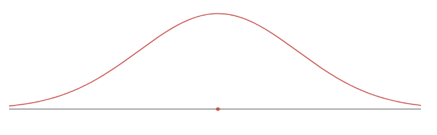
\includegraphics[width=3.36458in,height=\textheight]{images/img44.png}

Using R to compute cumulative probability for \(X \sim N(\mu, \sigma)\)

\begin{itemize}
\tightlist
\item
  For \(P(X < b) = P(X \leq b)\): \texttt{pnorm(b,\ \textbackslash{}mu,\ \textbackslash{}sigma)}
\item
  For \(P(X > a) = P(X \geq a)\): \texttt{pnorm(a,\ \textbackslash{}mu,\ \textbackslash{}sigma,\ lower.tail\ =\ FALSE)} or \texttt{1\ -\ pnorm(a,\ \textbackslash{}mu,\ \textbackslash{}sigma)}
\item
  For \(P(a < X < b)\): \texttt{pnorm(b,\ \textbackslash{}mu,\ \textbackslash{}sigma)\ -\ pnorm(a,\ \textbackslash{}mu,\ \textbackslash{}sigma)} or \texttt{1\ -\ (pnorm(a,\ \textbackslash{}mu,\ \textbackslash{}sigma)\ +\ pnorm(b,\ \textbackslash{}mu,\ \textbackslash{}sigma,\ lower.tail\ =\ FALSE))}
\item
  For \(Z \sim N(0, 1)\): the mean and SD can be omitted in 1)-3):

  \begin{itemize}
  \tightlist
  \item
    \(P(Z < b)\): \texttt{pnorm(b)}
  \end{itemize}
\end{itemize}

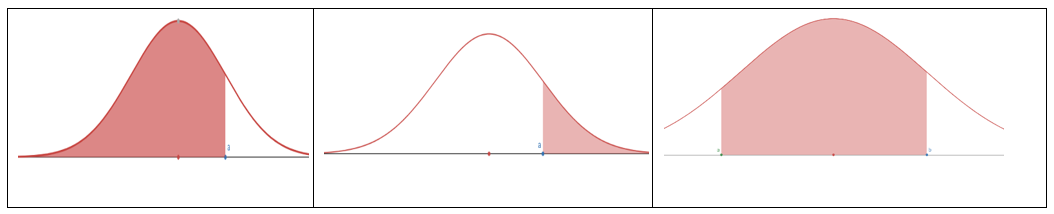
\includegraphics[width=5.72917in,height=\textheight]{images/img45.png}

\textbf{To Compute Inverse Cumulative Probability (Finding x for Given Cumulative Probability)}

\begin{itemize}
\tightlist
\item
  Find \(x\) for \(P(X < x) = p\): \texttt{qnorm(p,\ \textbackslash{}mu,\ \textbackslash{}sigma)}
\item
  Find \(x\) for \(P(X > x) = p\): \texttt{qnorm(1\ -\ p,\ \textbackslash{}mu,\ \textbackslash{}sigma)} or \texttt{qnorm(p,\ \textbackslash{}mu,\ \textbackslash{}sigma,\ lower.tail\ =\ FALSE)}
\end{itemize}

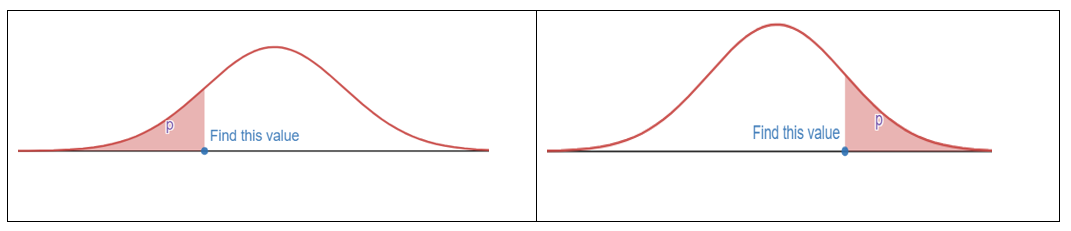
\includegraphics[width=5.72917in,height=\textheight]{images/img46.png}

\textbf{Z-score}

\begin{itemize}
\tightlist
\item
  If \(X \sim N(\mu, \sigma)\), the z-score of x is computed by \(z = \frac{x - \mu}{\sigma}\).
\item
  The z-score measures how many standard deviations of x from the mean.
\item
  \(Z = \frac{X - \mu}{\sigma} \sim N(0, 1)\)
\item
  \(X = \mu + Z \cdot \sigma\)
\item
  \(x = \mu\) if \(z = 0\); \(x > \mu\) if \(z > 0\); \(x < \mu\) if \(z < 0\)
\end{itemize}

\textbf{Empirical Rule (68-95-99.7 Rule)}

For a nearly normally distributed data, the empirical rule predicts that:

\begin{itemize}
\tightlist
\item
  68\% of observations fall within the first standard deviation (\(\mu\) ± \(\sigma\)).
\item
  95\% within the first two standard deviations (\(\mu\) ± 2\(\sigma\)).
\item
  99.7\% within the first three standard deviations (\(\mu\) ± 3\(\sigma\)) of the mean.
\end{itemize}

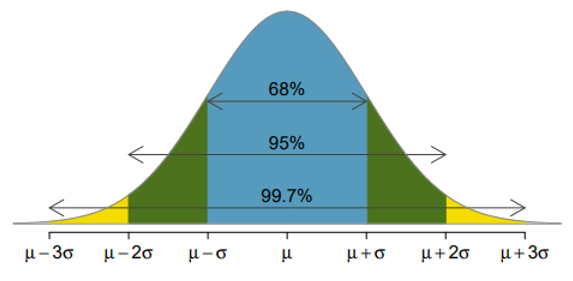
\includegraphics[width=4.25in,height=\textheight]{images/img47.png}

\textbf{Exercise 1} For \(Z \sim N(0, 1)\) (the standard normal distribution, the mean = 0, the standard deviation = 1), use R to find the probability and sketch the region that represents the probability.

(a). \(P(Z < -1.5)\) (b). \(P(Z > 1.75)\) (c). \(P(-1.5 < Z < 1.75)\) (d). \(P(|Z| < 2.5)\) (e). \(P(Z > 1)\)

\textbf{Exercise 2} For \(X \sim N(-3, 2)\) (the normal distribution, the mean = -3, the standard deviation = 2), use R to find the probability and sketch the region that represents the probability.

\begin{enumerate}
\def\labelenumi{\arabic{enumi}.}
\tightlist
\item
  \(P(X < -3.25)\)
\item
  \(P(X > 1.75)\)
\item
  \(P(-3.25 < X < -1.25)\)
\end{enumerate}

\textbf{Exercise 3} For \(X \sim N(-3, 2)\), compute the z-score of the given x:

\begin{enumerate}
\def\labelenumi{\arabic{enumi}.}
\tightlist
\item
  \(x = -3.25\)
\item
  \(x = -3\)
\item
  \(x = -1.25\)
\end{enumerate}

\textbf{Exercise 4}

(a). State the Empirical Rule.

(b). Use R to verify the Empirical Rule: find \(P(|Z| < 1)\), \(P(|Z| < 2)\), \(P(|Z| < 3)\).

\textbf{Exercise 5}

The scores on a college entrance exam follow a normal distribution with a mean of 50 and standard deviation of 10. Find the probability that a student will score:

(a). Over 65

(b). Less than 25

(c). Between 33 and 68

\textbf{Exercise 6}

The scores on a college entrance exam follow a normal distribution with a mean of 50 and standard deviation of 10.

(a). What is the cut off score of the lowest 20\%? (Round to 1 decimal)

(b). What is the cut off score of the highest 10\%? (Round to 1 decimal)

\textbf{Exercise 7}

The hours of sleep of college students fits a normal distribution with mean of 7.2 hours and standard deviation of 1.3 hours. Find the (standardized) z-score corresponding to 6.5 hours.

\textbf{Exercise 8}

John scored a 92 on a test with a mean of 88 and a standard deviation of 2.7. Jessica scored an 86 on a test with a mean of 82 and a standard deviation of 1.8. Find the Z-scores for John's and Jessica's test scores and use them to determine who did better on their test relativ*e to their class.

\textbf{Exercise 9}

The score data of the verbal portion of the Graduate Record Examination (GRE) is approximately normally distributed with a mean of 462 points and a standard deviation of 119 points. Fill in the following blanks: approximately

\emph{(a)} 68\% of students who took the verbal portion of the GRE scored between \_\_\_\_\_\_\_ and \_\_\_\_\_\_\_\_

\emph{(b)} 95\% of students who took the verbal portion of the GRE scored between \_\_\_\_\_\_ and \_\_\_\_\_\_\_\_

\emph{(c)} 99.7\% of students who took the verbal portion of the GRE scored between \_\_\_\_\_\_ and \_\_\_\_\_\_\_\_

\chapter{Inference for Proportion}\label{inference-for-proportion}

\textbf{Objective 1:} By the end of this unit, students will be able to:
::: \{.blue-background\}
- Understand the meaning of sampling distributions.
- Apply the central limit theorem to define the sampling distribution of a sample proportion.
- Identify the conditions needed for the central limit theorem to apply for sample proportions.
- Construct and interpret confidence intervals for the population proportion.
:::

\section{Point Estimates and Sampling Variability}\label{point-estimates-and-sampling-variability}

\textbf{Basic Terms}

\begin{itemize}
\tightlist
\item
  Sample proportion \(\hat{p} = \frac{x}{n}\)\\
\item
  Sample proportion \(\hat{p}\) is the unbiased point estimator for the population proportion \(p\)
\item
  A value of \(\hat{p}\) is a point estimate
\item
  Error = \(\hat{p} - p\)
\end{itemize}

\textbf{Central Limit Theorem (for Sampling Distribution of Sample Proportions)}

When observations are independent (take random samples of fixed size \(n\) without replacement); the sample size \(n\) is large enough, i.e.~\(np \geq 10\) and \(n(1-p) \geq 10\); and sample size \(n < 10\%\) of the population size then the sample proportion \(\hat{p}\) is approximately normal with mean = \(p\) and standard deviation = \(\sqrt{\frac{p(1-p)}{n}}\): \(\hat{p} \sim N(p, \sqrt{\frac{p(1-p)}{n}})\)

That is, \(z = \frac{\hat{p} - p}{\sqrt{\frac{p(1-p)}{n}}} \sim N(0, 1)\).

\textbf{Notes:}

\begin{itemize}
\item
  The requirement that the sample size \(n < 10\%\) of population size is to have the standard deviation \(\sqrt{\frac{p(1-p)}{n}}\).
\item
  If the sample size \(n < 10\%\) of population size, then the \(\sqrt{\frac{p(1-p)}{n}}\) is overly estimated SD, and the SD will typically adjust by a factor \(\sqrt{\frac{N-n}{N-1}}\),i.e.~\(\sqrt{\frac{N-n}{N-1}} \times \sqrt{\frac{p(1-p)}{n}}\).
\item
  When using \(\hat{p}\) to estimate \(p\), the Standard Error of \(\hat{p}\) is the standard deviation of its sampling distribution: \(S.E._{\hat{p}} = \sqrt{\frac{\hat{p}(1-\hat{p})}{n}}\)
\item
  When \(p\) is unknown, \(\hat{p}\) is used to replace \(p\) then check \(n\hat{p} \geq 10\) and \(n(1-\hat{p}) \geq 10\) (success and failure condition) estimated \(S.E. \approx \sqrt{\frac{\hat{p}(1-\hat{p})}{n}}\)
\end{itemize}

\textbf{Exercise 1}

In a random sample with size \(n=9000\), the count of ``yes'' is \(x=250\).

\emph{(a)} Compute the sample proportion \(\hat{p} = \frac{x}{n}\).

\emph{(b)} Compute the estimated standard error of the sample proportion \(S.E. \approx \sqrt{\frac{\hat{p}(1-\hat{p})}{n}}\).

\textbf{Exercise 2}

In a random sample of 765 adults in the U.S., 322 say they could not cover \$600 unexpected expense without borrowing money or going to debt.

\emph{(a)} What population is under consideration in the data set?

\emph{(b)} What parameter is being estimated?

\emph{(c)} Compute a point estimate for the parameter using the given information above?

\emph{(d)} What is the estimated standard error?

\textbf{Exercise 3}

Of all freshmen at a large college, 19\% made the dean's list.

\emph{(a)} What is the value of the interested parameter? State the sampling distribution of sample proportion for sample size 90.

\emph{(b)} If a random sample of 90 freshmen selected 14 made the dean's list. Compute the sample proportion and the Z-score.

\emph{(c)} If a random sample of 90 freshmen selected 20 made the dean's list. Compute the sample proportion and the Z-score.

\emph{(d)} What is the probability that at most 14 of selected 90 freshmen made the dean's list?

\emph{(e)} What is the probability that between 14 to 20 students of selected 90 freshmen made the dean's list?

\subsection{Point Estimate for Proportion}\label{point-estimate-for-proportion}

\textbf{Definition:}

A point estimate is the value of a statistic (based on a sample) that estimates the value of a population parameter.

Suppose we want to estimate the proportion of adult Americans who believe that immigration is a good thing for the U.S. It is unreasonable to expect that we could survey every adult American. Instead, we use a sample of adult Americans to arrive at an estimate of the proportion. We call this estimate a point estimate.

\textbf{The sample proportion} \(\hat{p}\)

We now study categorical data and draw inference on the proportion, or percentage, of the population with a specific characteristic.\\
If we call a given categorical characteristic in the population ``success'' then the sample proportion of successes, p, is:

\[\hat{p}= \frac{x}{n} \]

Where x is the number of individuals in the sample with a specified characteristic and n is the sample size.

\textbf{Example 1:} The Gallup Organization conducted a poll in which a simple random sample of 1,520 adults, living in all 50 U.S. states and the District of Columbia were asked the following question. ``Thinking now about immigrants -- that is, people who come from other countries to live here in the United States, in your view, do you think legal immigration is a good thing or a bad thing for this country today?'' If 1135 responded ``Yes''.

Obtain a point estimate for the proportion of Americans 18 and older who believe that immigration is good for the US.

\textbf{Solution:}

\[\hat{p}= \frac{1135}{1520} = 0.747\]

We estimate for the proportion of Americans 18 and older who believe that immigration is good for the US is 74.7\%\\
\textbf{Note:} We agree to round proportions to three decimal places.

\textbf{Sampling distribution of sample proportions} \(\hat{p}\)

\subsection{The Central Limit Theorem for proportions}\label{the-central-limit-theorem-for-proportions}

The Central Limit Theorem for proportions states that if n is large enough, then:

\(\hat{p}\sim N \left( p, \sqrt{\frac{p(1-p)}{n}} \right)\)

Therefore, a different random sample of adult Americans might result in a different point estimate of the population proportion, such as \(\hat{p}= 0.71, \hat{p}= 0.78, \ldots\).

If the method used to select the sample of Americans was done appropriately, both point estimates would be good guesses of the population proportion. Due to variability in the sample proportion, we need to report a range (or \emph{interval}) of values, including a measure of the likelihood that the interval includes the unknown population proportion.

\subsection{Confidence Interval}\label{confidence-interval}

\textbf{Quick Review on Confidence Interval}

About critical value \(z^*\) or \(z_{\alpha/2}\): For \(N(0,1)\), \(z_{\alpha/2}\) is the cut-off point with upper tail of probability \(\alpha/2\)

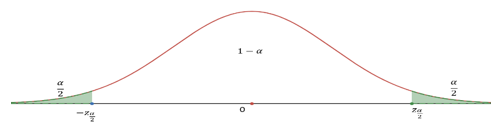
\includegraphics[width=3.64583in,height=1.14583in]{images/img48.png}

\textbf{How to find} \(z_{\alpha/2}\):

\begin{enumerate}
\def\labelenumi{(\arabic{enumi})}
\item
  For \(100(1-\alpha)\%\) confidence level, find \(\alpha\) then \(\alpha/2\)
\item
  Use R: \(qnorm\left(\frac{\alpha}{2}, \text{lower.tail} = \text{FALSE}\right)\) or \(qnorm\left(1 - \frac{\alpha}{2}\right)\)
\end{enumerate}

\textbf{Common} \(z_{\alpha/2}\) values:

\begin{longtable}[]{@{}lll@{}}
\toprule\noalign{}
Confidence level & \(\alpha\) & \(z_{\alpha/2}\) \\
\midrule\noalign{}
\endhead
\bottomrule\noalign{}
\endlastfoot
90\% & 0.10 & \(z_{0.05} = 1.644854 \approx 1.645\) \\
95\% & 0.05 & \(z_{0.025} = 1.959964 \approx 1.96\) \\
98\% & 0.02 & \(z_{0.01} = 2.326348 \approx 2.326\) \\
99\% & 0.01 & \(z_{0.005} = 2.575829 \approx 2.576\) \\
\end{longtable}

\textbf{Construct} \(100(1-\alpha)\%\) confidence interval: Use \(\hat{p}\), \(n\), and \(z_{\alpha/2}\)

\(\hat{p} \pm z_{\alpha/2} \times \sqrt{\frac{\hat{p}(1-\hat{p})}{n}}\) (or \((\hat{p} - z_{\alpha/2} \times \sqrt{\frac{\hat{p}(1-\hat{p})}{n}}, \hat{p} + z_{\alpha/2} \times \sqrt{\frac{\hat{p}(1-\hat{p})}{n}})\))

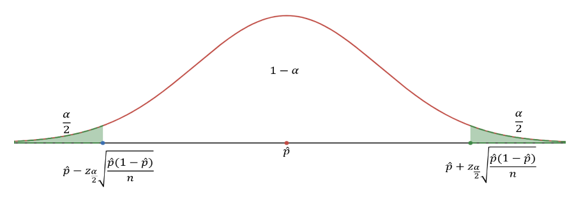
\includegraphics[width=4.44792in,height=\textheight]{images/img50.png}

\textbf{Margin of Error (M.E.)}

\(M.E. = z_{\alpha/2} \times \sqrt{\frac{\hat{p}(1-\hat{p})}{n}}\)

So, C.I.: point estimate \(\pm M.E.\)

Note: the point estimate is the middle point; the \(M.E.\) = half of the length of C.I.)

\textbf{Interpretation of C.I.:}

With the confidence level of \(100(1-\alpha)\%\) and a sample proportion \(\hat{p}\) with sample size \(n\), we are \(100(1-\alpha)\%\) confident that the population proportion \(p\) is in the confidence interval \((\hat{p} - z_{\alpha/2} \times \sqrt{\frac{\hat{p}(1-\hat{p})}{n}}, \hat{p} + z_{\alpha/2} \times \sqrt{\frac{\hat{p}(1-\hat{p})}{n}})\)

\textbf{Minimum sample size to guarantee the specified} \(M.E. \leq a\)

For known \(p\): \(n = \text{ceiling} \left[ \frac{p(1-p) \times z_{\alpha/2}^2}{a^2} \right]\)

For unknown \(p\): \(n = \text{ceiling} \left[ \frac{1}{4} \times \frac{z_{\alpha/2}^2}{a^2} \right]\)

\textbf{Exercise 1}

\emph{(a)} Construct a 95\% confidence interval using a sample proportion \(\hat{p} = 0.3\) and sample size \(n=1000\).

\emph{(b)} Construct a 90\% confidence interval using a sample proportion \(\hat{p} = 0.3\) and sample size \(n=1000\).

\emph{(c)} Construct a 95\% confidence interval using a sample proportion \(\hat{p} = 0.3\) and sample size \(n=100\).

\textbf{Exercise 2}. Circle the proper choices.

\emph{(a)} The confidence interval is \_\_\_\_\_\_\_\_\_\_\_(wider/narrower) if the sample size is increasing.

\emph{(b)} The confidence interval is \_\_\_\_\_\_\_\_\_\_\_(wider/narrower) if the confidence level is increasing.

\textbf{Exercise 3}

\emph{(a)} Construct a 98\% confidence interval using a sample proportion 45\% and standard error 1.2\%. (Assume that the CLT can be applied)

\emph{(b)} Compute the margin of error using the same information of (a).

\textbf{Exercise 4}

A website is trying to increase registration of first-time visitors using a new site design. Of 752 randomly sampled visitors over a month who saw the new design, 64 registered.

\emph{(a)} Compute the sample proportion.

\emph{(b)} Compute the standard error.

\emph{(c)} Construct and interpret a 90\% confidence interval for the fraction of first-time visitors of the site who would register under the new design.

\textbf{Exercise 5}. For a confidence interval of proportion \((0.291, 0.309)\) find the following:

\emph{(a)} The sample proportion that was used to create this C.I.

\emph{(b)} The M.E. (Margin of Error)

\textbf{Exercise 6}

A public health survey is going to estimate the proportion of a population \(p\) having defective vision. How many persons should be examined if the public health commissioner wishes to be 95\% certain that the margin of error is below 0.04 when:

\emph{(a)} \(p\) is known to be about 0.45.

\emph{(b)} There is no knowledge about the value of \(p\)?

\textbf{Note}. Similar result for mean:

\begin{itemize}
\item
  CLT: In random sampling from a population with mean \(\mu\) and standard deviation \(\sigma\), when the sample size \(n\) is large (\(n \geq 30\)), the distribution of sample mean \(\bar{X}\) is approximately normal: \(\bar{X} \sim N(\mu, \frac{\sigma}{\sqrt{n}})\).
\item
  Use \(\bar{x}\) as point estimate for \(\mu\).
\item
  \(S.E. = \frac{\sigma}{\sqrt{n}} \approx \frac{s}{\sqrt{n}}\)
\item
  \(100(1-\alpha)\%\) confidence interval for mean: \(\bar{x} \pm z_{\alpha/2} \times \sqrt{\frac{s}{n}}\) or \((\bar{x} - z_{\alpha/2} \times \sqrt{\frac{s}{n}}, \bar{x} + z_{\alpha/2} \times \sqrt{\frac{s}{n}})\)
\item
  \(M.E. = z_{\alpha/2} \times S.E. = z_{\alpha/2} \times \sqrt{\frac{s}{n}}\)
\end{itemize}

\textbf{Exercise 7}

The GSS (General Social Survey) asked the question: ``For how many days during the past 30 days was your mental health not good (stress, depression, with emotions)?'' Based on responses from 1151 US residents, a 95\% confidence interval (3.40, 4.24) (days) was reported in 2014.

\emph{(a)} Determine the sample mean (days).

\emph{(b)} Determine the margin of error (M.E.).

\emph{(c)} What is the value of \(z_{\alpha/2}\) for 95\% confidence level?

\emph{(d)} Write a sentence to interpret this confidence interval.

\subsection{Confidence Intervals for Proportion}\label{confidence-intervals-for-proportion}

A confidence interval for an unknown parameter consists of an interval of numbers based on a point estimate.

The level of confidence represents the expected proportion of intervals that will contain the parameter if a large number of different samples is obtained.

The level of confidence is denoted \((1 - \alpha) \times 100\%\). For example, a 95\% level of confidence \((\alpha = 0.05)\) implies that if 100 different confidence intervals are constructed, each based on a different sample from the same population, we will expect 95 of the intervals to contain the parameter and 5 not to include the parameter.

Confidence interval estimates for the population proportion are of the form:

\textbf{Point estimate} \(\pm\) \textbf{margin of error.}

The margin of error of a confidence interval estimate of a parameter is a measure of how accurate the point estimate is. The margin of error depends on three factors:

\begin{itemize}
\item
  \textbf{Level of confidence:} As the level of confidence increases, the margin of error also increases.
\item
  \textbf{Sample size:} As the size of the random sample increases, the margin of error decreases.
\item
  \textbf{Standard deviation of the population:} The more spread there is in the population, the wider our interval will be for a given level of confidence.
\item
  \textbf{Point estimate}

  \begin{itemize}
  \tightlist
  \item
    statistics vs.~parameter
  \item
    point estimate for population proportion is \(\hat{p}=\frac{x}{n}\)
  \item
    may also represent a probability of a binomial distribution, such as p=0.5 for a fair coin.
  \end{itemize}
\item
  \textbf{Confidence interval} for an unknown parameter
\item
  \textbf{Margin of error}
\item
  Interpretation of what is meant by being ``95\%'' confident (think simulations)
\item
  Formula for confidence interval for population proportion, p.
\item
  Know z - multipliers for 90\%, 95\%, and 99\% confidence intervals.
\item
  Requirements:

  \begin{itemize}
  \item
    Random sample (independent)
  \item
    AND large sample size (at least 10 successes \(\&\) 10 Failures) np\textgreater10 and n(1-p) \textgreater{} 10
  \item
    Calculating sample size to obtained desired margin of error E.

    \begin{itemize}
    \tightlist
    \item
      Using educated guess for population proportion.
    \item
      Using p=0.5 for conservative (large) sample size.
    \end{itemize}
  \item
    Round up to nearest integer.
  \end{itemize}
\end{itemize}

Suppose that a simple random sample of size \(n\) is taken from a population.\\
A \((1 - \alpha) \times 100\%\) confidence interval for p is given by the following quantities:

\(\hat{p}\pm z^* \times \sqrt{\frac{\hat{p}(1-\hat{p})}{n}}\)

Where p = Theoretical or ``True'' population proportion

\begin{longtable}[]{@{}
  >{\raggedright\arraybackslash}p{(\columnwidth - 6\tabcolsep) * \real{0.2338}}
  >{\raggedright\arraybackslash}p{(\columnwidth - 6\tabcolsep) * \real{0.3506}}
  >{\raggedright\arraybackslash}p{(\columnwidth - 6\tabcolsep) * \real{0.1299}}
  >{\raggedright\arraybackslash}p{(\columnwidth - 6\tabcolsep) * \real{0.2857}}@{}}
\toprule\noalign{}
\begin{minipage}[b]{\linewidth}\raggedright
Confidence Level
\end{minipage} & \begin{minipage}[b]{\linewidth}\raggedright
\(1 - \alpha \times 100\%\)
\end{minipage} & \begin{minipage}[b]{\linewidth}\raggedright
\(\alpha\)
\end{minipage} & \begin{minipage}[b]{\linewidth}\raggedright
\(Z^* = Z_{\alpha/2}\)
\end{minipage} \\
\midrule\noalign{}
\endhead
\bottomrule\noalign{}
\endlastfoot
0.90 & 0.10 & 1.645 & \\
0.95 & 0.05 & 1.96 & \\
0.98 & 0.02 & 2.33 & \\
0.99 & 0.01 & 2.58 & \\
\end{longtable}

The Z-table is used to find the critical values, \(Z^*\), for confidence intervals on the true proportion p.~This abbreviated table gives the most common z-scores for the centered values of confidence for the normal curve.

\textbf{Example 2:}

In July of 2008, a University Poll asked 1783 registered voters nationwide whether they favored or opposed the death penalty for persons convicted of murder 1123 were in favor.

Obtain a 90\% confidence interval for the proportion of registered voters nationwide who are in favor of the death penalty for persons convicted of murder.

\textbf{Solution:}\\
\(\hat{p} = \frac{1123}{1783} = 0.63\)

Where:

n = 1783

\[
np \ \& \ n(1-p) > 10
\]

Lower bound: \(0.63 - 1.645 \times \sqrt{\frac{0.63(1-0.63)}{1783}} \approx 0.61\)\\
Upper bound: \(0.63 + 1.645 \times \sqrt{\frac{0.63(1-0.63)}{1783}} \approx 0.65\)

We are 90\% confident that the proportion of registered voters who are in favor of the death penalty for those convicted of murder is between 0.61 and 0.65.

\textbf{Estimating the margin of error on p for a given confidence level}

Consider the scenarios for the product of proportion and complements for the margin of error. What happens as the proportion changes?

\[
(1 - \alpha)\% CI \text{ on } p = \hat{p} \pm Z_{\frac{\alpha}{2}} \sqrt{\frac{\hat{p}(1-\hat{p})}{n}}
\]

Where:

\begin{itemize}
\tightlist
\item
  \(\hat{p}\) = Point estimate
\item
  \(Z_{\frac{\alpha}{2}} \sqrt{\frac{\hat{p}(1-\hat{p})}{n}}\) = Margin of Error = \(Z_{critical} \times Standard Error\)
\end{itemize}

Determine the Sample Size Necessary for Estimating a Population Proportion within a Specified Margin of Error

Two possible solutions:

\begin{enumerate}
\def\labelenumi{\arabic{enumi}.}
\tightlist
\item
  Use an estimate of p based on a pilot study
\item
  Use the value of p which gives the largest possible value of \(n\) for a given confidence level \(\&\) margin of error.
\end{enumerate}

\textbf{Sample Size Needed for Estimating the Population Proportion}

The sample size required to obtain a \((1 - \alpha)\) - 100\% confidence interval for \(p\) with a margin of error E is given by:

\[
n = \frac{p(1-p) \left( \frac{Z_{\frac{\alpha}{2}}}{E} \right)^2}{rounded \text{ up to the next integer}}, \text{ where } p \text{ is a prior estimate of } p.
\]

\begin{longtable}[]{@{}ll@{}}
\toprule\noalign{}
\(n\) & Approximate Margin of Error \\
\midrule\noalign{}
\endhead
\bottomrule\noalign{}
\endlastfoot
500 & 0.045 (or 4.5\%) \\
800 & 0.035 (or 3.5\%) \\
1000 & 0.032 (or 3.2\%) \\
1500 & 0.026 (or 2.6\%) \\
\end{longtable}

If a prior estimate on the proportion is unavailable, using \(\hat{p} = 0.5\) will give the following estimate for the sample size:

\[
n = 0.25 \times \left( \frac{Z_{\frac{\alpha}{2}}}{E} \right)^2
\]

Gallup and other polling agencies report at the 95\% confidence level and assume p = 0.5 in calculating the margin of error:

\textbf{Example 3}

The statistic presented below appeared in the weekly magazine TIME, August 23, 1993, under the article \emph{Danger in the Safety Zone}. Consider the tiny print ``From telephone poll of 500 adult Americans taken for TIME/CNN. Margin of error is \(\pm 0.45\)''.

Do you favor the death penalty?

\begin{longtable}[]{@{}ll@{}}
\toprule\noalign{}
YES & NO \\
\midrule\noalign{}
\endhead
\bottomrule\noalign{}
\endlastfoot
77\% & 17\% \\
\end{longtable}

From a telephone poll of 500 adult Americans taken for TIME/CNN on Aug.~12 by Yankelovich Partners, Inc.~Margin of error is \(\pm 0.45\)

Explain how the margin of error can be calculated.

Solution: Margin of Error in the article (under 95\% confidence) is about:

\[
1.96 \sqrt{\frac{0.5 \times 0.5}{500}} \approx \frac{1}{\sqrt{500}} = 0.04472 \approx 4.5\%
\]

\textbf{Example 2 Illustrating the Meaning of Level of Confidence Using Simulation :}

Let's illustrate what ``95\% confidence'' means in a 95\% confidence interval in another way. We will simulate obtaining 200 different random samples of size n=50, m=50 i.e., n equals 50 from a population with p=0.7, p equals 0.7. Figure 4 shows the confidence intervals in groups of 100. A green interval is a 95\% confidence interval that includes the population proportion, 0.7. A red interval is a confidence interval that does not include the population proportion. (For now, ignore the blue intervals.) Notice that the red intervals that do not capture the population proportion 0.7 have centers that are far away (more than 1.96 standard errors) from 0.7. Of the 200 confidence intervals obtained, 10 (the red intervals) do not include the population proportion. For example, the first interval to miss has a sample proportion that is too small to result in an interval that captures 0.7.

(Note: The actual image illustrating the confidence intervals would be embedded here using \(\text{![ ]()}\) if the image file was provided.)

\textbf{Appeal: Simulating Confidence Intervals (rossmanchance.com)}

A 95\% level of confidence means that 95\% of all possible samples result in confidence intervals that include the parameter (and 5\% of all possible samples result in confidence intervals that do not include the parameter).

\textbf{Caution!}

A 95\% confidence interval does \emph{not} mean that there is a 95\% probability that the interval contains the parameter (such as p). Remember, probability describes the likelihood of \emph{undetermined} events. Therefore, it does not make sense to talk about the probability that the interval contains the parameter since the parameter is a \emph{fixed} value. Thinking of this way: If a coin and obtain a head. If I ask you to determine the probability that the flip resulted in a head, it would not be 0.5, because the outcome has already been determined. Instead, the probability is 0 or 1. Confidence intervals work the same way. Because p or \(\mu\) is already determined, we do not say that there is a 95\% probability that the interval contains \(\mu\).

\textbf{Exercises}

\begin{enumerate}
\def\labelenumi{\arabic{enumi}.}
\item
  As a potential worldwide pandemic, avian influenza H5N1 (commonly called the bird flu) poses a serious health risk. As of January 24, 2012, there have been 583 human cases of this virus in the world. Of these cases, 344 have resulted in death. Consider the outcomes of these cases as a random sample of all possible outcomes.

  \begin{enumerate}
  \def\labelenumii{\alph{enumii}.}
  \tightlist
  \item
    Find a point estimate for the proportion of people who would die if infected with the bird flu.
  \item
    Construct a 90\% confidence interval for the proportion of cases that would be expected to result in death if a pandemic occurred.
  \item
    Interpret the confidence interval.
  \end{enumerate}
\item
  A sociologist wanted to determine the percentage of residents of America that only speak English at home. What size sample should be obtained if she wishes her estimate to be within 3 percentage points with 90\% confidence assuming she uses the estimate obtained from the Census 2000 Supplementary Survey of 82.4\%?
\item
  Nitrates are groundwater contaminants derived from fertilizer, septic tank seepage, and other sewage. Nitrate poisoning is particularly hazardous to infants under the age of 6 months. The Maximum Contaminant Level (MCL) is the highest level of a contaminant that government allows in drinking water. For nitrates, the MCL is 10 mg/L. The health department wants to know the proportion of wells in Madison County that have nitrate levels above the MCL. A worker has been assigned to take a simple random sample of wells in the county, measure the nitrate levels, and assess compliance. What size sample should the health department obtain if the estimate is desired to be within 2 percent with 95\% confidence if:

  \begin{enumerate}
  \def\labelenumii{\alph{enumii}.}
  \tightlist
  \item
    there is no prior information available?
  \item
    a study conducted two years ago showed that approximately 7\% of the wells in Madison County had nitrate levels exceeding the MCL.
  \end{enumerate}
\end{enumerate}

\subsection{Confidence interval for two-sided test}\label{confidence-interval-for-two-sided-test}

For \(H_0: p = p_0\), \(H_a: p \neq p_0\) (two-sided) and significance level \(\alpha\), construct a \(100(1-\alpha)\%\) confidence interval: \(\hat{p} \pm z_{\alpha/2} \times \sqrt{\frac{\hat{p}(1-\hat{p})}{n}}\)

Make decision:

\begin{itemize}
\tightlist
\item
  If \(p_0\) is not in the C.I. then we reject \(H_0\) in favor of \(H_a\);
\item
  If \(p_0\) is in the C.I. then we fail to reject \(H_0\).
\end{itemize}

\textbf{Type I and Type II errors}

\begin{longtable}[]{@{}
  >{\raggedright\arraybackslash}p{(\columnwidth - 6\tabcolsep) * \real{0.1463}}
  >{\raggedright\arraybackslash}p{(\columnwidth - 6\tabcolsep) * \real{0.2073}}
  >{\raggedright\arraybackslash}p{(\columnwidth - 6\tabcolsep) * \real{0.2561}}
  >{\raggedright\arraybackslash}p{(\columnwidth - 6\tabcolsep) * \real{0.3902}}@{}}
\toprule\noalign{}
\begin{minipage}[b]{\linewidth}\raggedright
Truth
\end{minipage} & \begin{minipage}[b]{\linewidth}\raggedright
Test conclusion
\end{minipage} & \begin{minipage}[b]{\linewidth}\raggedright
do not reject \(H_0\)
\end{minipage} & \begin{minipage}[b]{\linewidth}\raggedright
reject \(H_0\) in favor of \(H_A\)
\end{minipage} \\
\midrule\noalign{}
\endhead
\bottomrule\noalign{}
\endlastfoot
\(H_0\) true & & okay & Type 1 Error \\
\(H_A\) true & & Type 2 Error & okay \\
\end{longtable}

\textbf{Example}

Claim: \(p<0.32\), \(n=120\), \(p=0.233\), \(\alpha=0.05\)

\textbf{Solution}

\emph{(a)} Formulate the hypotheses: \(H_0: p=0.32\), \(H_a: p<0.32\)

\emph{(b)} Compute the \(z\)-test statistic: \(z = \frac{0.233-0.32}{\sqrt{\frac{0.32 \times 0.68}{120}}} = -2.043057\) (R-code: \texttt{(0.233-0.32)/sqrt(0.32*0.68/120)})

\emph{(c)} Compute the p-value: p-value \(= P(Z < -2.043057) = 0.020534\) (R-code: \texttt{pnorm(-2.043057)})

\emph{(d)} Draw conclusion: since the p-value is less than \(\alpha\), \(0.0205 < 0.05\), we reject the null hypothesis and support the alternative hypothesis: We have strong evidence to support the claim that the proportion is less than 0.32 (\(p<0.32\)).

Do the following hypotheses testing for given claims, sample size, sample proportion, and significance level:

\begin{enumerate}
\def\labelenumi{\arabic{enumi}.}
\item
  Claim: \(p<0.56\), \(n=86\), \(\hat{p}=0.387\), \(\alpha=0.10\)
\item
  Claim: \(p>0.75\), \(n=228\), \(\hat{p}=0.818\), \(\alpha=0.02\)
\item
  Claim: \(p \neq 0.60\), \(n=77\), \(\hat{p}=0.709\), \(\alpha=0.02\)
\item
  Claim: \(p \neq 0.60\), \(n=77\), \(\hat{p}=0.565\), \(\alpha=0.02\)
\end{enumerate}

\section{\texorpdfstring{Hypothesis Testing for \(p\)}{Hypothesis Testing for p}}\label{hypothesis-testing-for-p}

\textbf{Learning Objectives:}

\textbf{Objective 2:} By the end of this unit, students will be able to:

\begin{itemize}
\tightlist
\item
  Formulate claims about a population proportion in the form of a null hypothesis and alternative hypothesis.
\item
  Identify the types of errors associated with statistical hypothesis testing.
\item
  Conduct a large-sample z-test about population proportions.
\end{itemize}

\textbf{Hypothesis Testing Steps}

\begin{enumerate}
\def\labelenumi{\arabic{enumi}.}
\tightlist
\item
  Formulate the null hypothesis and the alternative hypothesis
\item
  Use sample to compute p-value (or compute the test statistic and use the rejection region based on given significance level)
\item
  Make decision for specified significance level
\end{enumerate}

\textbf{Formulation of Hypothesis}

\textbf{The null hypothesis:} \(H_0: p = p_0\)

\textbf{The alternative hypothesis is one of the three:}

\begin{itemize}
\tightlist
\item
  \(H_a: p > p_0\) (right-sided) (or right-tailed)
\item
  \(H_a: p < p_0\) (left-sided) (or left-tailed)
\item
  \(H_a: p \neq p_0\) (two-sided) (or two-tailed)
\end{itemize}

\textbf{What is p-value}

A p-value is the calculated probability of observing data at least as favorable to the alternative hypothesis, assuming that the null hypothesis is true (in this section, we use the observed \(\hat{p}\), and under assumption the sample proportion \(\sim N(p_0, \sqrt{\frac{p_0(1-p_0)}{n}})\))

\textbf{How to compute p-value}

Use a sample of sample size \(n\) with sample proportion \(\hat{p}=p_1\), under the assumption that:

\(\hat{p}\) \(\sim N(p_0, \sqrt{\frac{p_0(1-p_0)}{n}})\)).

Let \(z_1 = \frac{p_1 - p_0}{\sqrt{\frac{p_0(1-p_0)}{n}}}\) (this is called the \(z\)-test statistic)

\begin{itemize}
\tightlist
\item
  For left-sided test, p-value is \(P(\hat{p} < p_1)\), or \(P(Z < z_1)\),
\end{itemize}

use pnorm \(({p_1, p_0,}{\sqrt{\frac{p_0(1-p_0)}{n}}})\) or pnorm \((z_1)\)

\begin{itemize}
\tightlist
\item
  For right-sided test, p-value is \(P(\hat{p} > p_1)\), or \(P(Z > z_1)\), use pnorm\(({p_1,p_0,}{\sqrt{\frac{p_0(1-p_0)}{n}}}, lower.tail = FALSE)\) or
\end{itemize}

pnorm \((z_1, lower.tail = FALSE)\)

\begin{itemize}
\tightlist
\item
  For two-sided test, p-value is \(P(|Z| > |z_1|)\), use 2*pnorm \((-|z_1|)\) or
\end{itemize}

2*pnorm \((|z_1|, lower.tail = FALSE)\)

\textbf{Make decision by comparing p-value with significance level} \(\alpha\)

\begin{itemize}
\item
  If p-value \(\leq \alpha\), then we have enough evidence to reject \(H_0\) and substantiate \(H_a\);
\item
  If p-value \(> \alpha\), then we do not have enough evidence to reject \(H_0\)
\item
  The default value of significance level is \(\alpha = 0.05\)
\end{itemize}

\textbf{Exercise 1}

Formulate the null and alternative hypotheses in the following situations:

\emph{(a)} A company claims that the proportion of its customers that have complaints against the company is now less than 0.13.

\emph{(b)} An inspector wants to establish that 2×4 lumber at a mill does not meet a specification that requires at most 5\% break under a standard load.

\emph{(c)} A university official believes that the proportion of students who currently hold part-time jobs has changed from the value 0.26 that prevailed four years ago.

\textbf{Exercise 2}

A census recorded five years ago that 20\% of the families in a large community lived below the poverty level. To determine if this percentage has changed, a random sample of 400 families is studied and 70 are found to be living below the poverty level. Does this finding indicate that the current percentage of families earning income below the poverty level has changed from what it was five years ago? (Use significance level \(\alpha=0.05\))

Follow the steps to conduct the hypotheses testing:

\emph{(a)} Formulate the hypotheses

\emph{(b)} Compute the sample proportion

\emph{(c)} Compute the test statistic

\emph{(d)} Compute the p-value

\emph{(e)} Draw conclusion using the significance level \(\alpha=0.05\).

\textbf{Exercise 3}

Conduct hypotheses testing.

Follow the example (Please redo the example by yourself)

\chapter{Inference for Mean}\label{inference-for-mean}

\textbf{Objective 1:} By the end of this unit, students will be able to:

\begin{itemize}
\tightlist
\item
  Distinguish between normal distribution and t distribution.
\item
  Compute point estimates and confidence intervals for estimating one population mean based on one sample and paired samples.
\item
  Formulate claims about a population mean in the form of a null hypothesis and alternative hypothesis.
\item
  Conduct t-tests for testing claims about a single population mean based on one sample and paired samples.
\end{itemize}

\section{Quick Review on Inference for Mean}\label{quick-review-on-inference-for-mean}

\begin{itemize}
\tightlist
\item
  Sample mean \(\bar{x}\) is the unbiased \textbf{point estimator} for the population mean \(\mu\)
\item
  A value of \(\bar{x}\) is a point estimate
\item
  Error = \(\mu - \bar{x}\)
\end{itemize}

\section{Central Limit Theorem (Sampling distribution of sample mean)}\label{central-limit-theorem-sampling-distribution-of-sample-mean}

When taking samples of fixed size \(n\) from a population with mean \(\mu\) and standard deviation \(\sigma\), when the observations are independent (take random samples of fixed size \(n\), without replacement); the sample size \(n \geq 30\), then the sample proportion \(\bar{x}\) is approximately normal: \(\bar{x} \sim N(\mu, \frac{\sigma}{\sqrt{n}})\).

When we know the population is normal, no matter what sample size, \(\bar{x} \sim N(\mu, \frac{\sigma}{\sqrt{n}})\)

\textbf{Notes:}

\begin{itemize}
\tightlist
\item
  When using \(\bar{x}\) to estimate \(\mu\) the Standard Error of \(\bar{x}\) is the standard deviation of its sampling distribution: \(S.E. = \frac{\sigma}{\sqrt{n}}\)
\item
  Usually \(\sigma\) is unknown use \(s\) to replace \(\sigma\): \(S.E. \approx \frac{s}{\sqrt{n}}\)
\end{itemize}

\textbf{When can the CLT be applied}

\begin{itemize}
\tightlist
\item
  If \(n \geq 30\) and \(\sigma\) is known
\item
  If the population is normal and \(\sigma\) is known
\item
  Otherwise we use t-distribution: \(T = \frac{\bar{x} - \mu}{s/\sqrt{n}} \sim t_{df}\), where \(df=n-1\) is the degree of freedom.
\end{itemize}

\textbf{t-distribution}

Similar to the standard normal distribution: the probability density curve of a t-distribution is centered at 0, and it is bell-shaped. But tails of a t-distribution are thicker than that of the standard normal distribution; moreover, the lower \(df\), the thicker the tails.

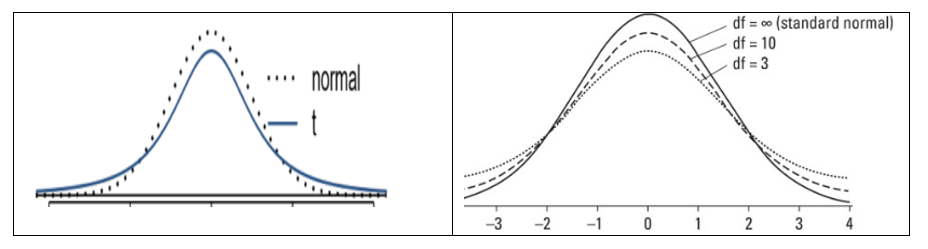
\includegraphics[width=5.20833in,height=\textheight]{images/img52.png}

\textbf{Using R to find probability under t-distribution with} \(df=n-1\):

\begin{itemize}
\tightlist
\item
  For \(P(T < b)\): \texttt{pt(b,\ df)}
\item
  For \(P(T > a)\): \texttt{pt(a,\ df,\ lower.tail\ =\ FALSE)} or \texttt{1\ -\ pt(a,\ df)}
\item
  For \(P(a < T < b)\): \texttt{pt(b,\ df)\ -\ pt(a,\ df)}
\end{itemize}

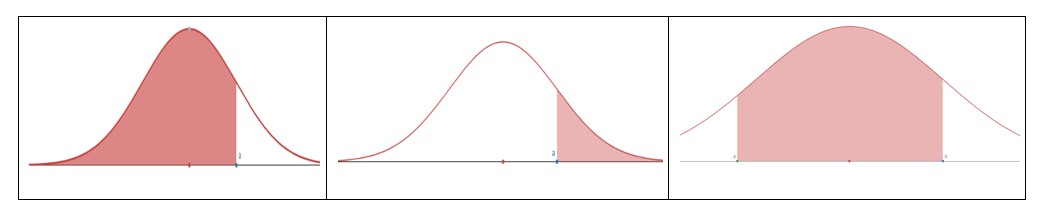
\includegraphics[width=5.72917in,height=\textheight]{images/img53.png}

\textbf{To find the cut-off point} \(t\) (critical value \(t^*\) or \(t_{\alpha/2}\)) for a given cumulative probability with \(df=n-1\):

\begin{itemize}
\tightlist
\item
  Find \(t\) for \(P(T < t) = p\): \texttt{qt(p,\ df)}
\item
  Find \(t\) for \(P(T > t) = p\): \texttt{qt(1\ -\ p,\ df)} or \texttt{qt(p,\ df,\ lower.tail\ =\ FALSE)}
\item
  \(t_{\alpha/2}\): \(P(T > t_{\alpha/2})\) = \(\alpha/2\): \(qt(\alpha/2, df, lower.tail = FALSE)\)
\end{itemize}

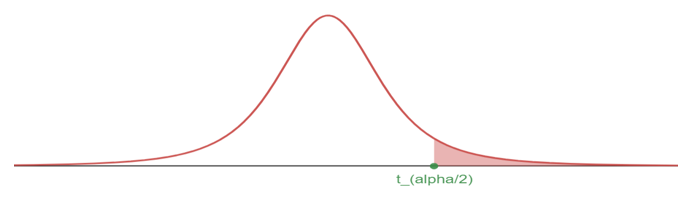
\includegraphics[width=5.20833in,height=\textheight]{images/img54.png}

\textbf{100}\((1-\alpha)\%\) Confidence interval for mean \(\mu\)

Using sample with size \(n\), sample mean \(\bar{x}\), sample standard deviation \(s\), the critical value \(t_{\alpha/2}\): \(\bar{x} \pm t_{\alpha/2} \times \frac{s}{\sqrt{n}}\)

\textbf{Margin of Error (M.E.)}

\(M.E. = t_{\alpha/2} \times S.E. = t_{\alpha/2} \times \frac{s}{\sqrt{n}}\)

\textbf{Hypothesis Testing for mean} \(\mu\) -- one sample t test (Same framework as the Hypothesis Testing for proportion)

\textbf{Steps:}

\begin{enumerate}
\def\labelenumi{\arabic{enumi}.}
\item
  Set up the hypotheses
\item
  Compute the t test statistic

  Using sample with size \(n\), sample mean \(\bar{x}\), sample standard deviation \(s\), null value \(\mu_0\),

  \(T = \frac{\bar{x} - \mu_0}{s/\sqrt{n}}\)
\item
  Compute the p-value

  Let t-test statistic \(t_1 = \frac{\bar{x} - \mu_0}{s/\sqrt{n}}\) (from step 2)

  \begin{itemize}
  \item
    For left-sided test, p-value is \(P(T < t_1)\) use \texttt{pt(t,\ df)}
  \item
    For right-sided test, p-value is \(P(T > t_1)\) use \texttt{pt(t,\ df,\ lower.tail\ =\ FALSE)}
  \item
    For two-sided test, p-value is \(P(|T| > |t_1|)\) use \(2*pt(-|t_1|, df)\) or \(2*pt(|t_1|, df, lower.tail = FALSE)\)
  \end{itemize}
\item
  Compare the p-value with the significance level \(\alpha\) and make decision

  \begin{itemize}
  \item
    If p-value \(\leq \alpha\), then we have enough evidence to reject \(H_0\) and substantiate \(H_a\);
  \item
    If p-value \textgreater{} \(\alpha\), then we do not have enough evidence to reject \(H_0\)
  \item
    The default value of significance level is \(\alpha = 0.05\)
  \end{itemize}
\end{enumerate}

\textbf{Exercise 1}

Without finding the values, arrange the numbers from small to large:

\begin{enumerate}
\def\labelenumi{\alph{enumi})}
\tightlist
\item
  \(P(Z < -1.25)\)\\
\item
  \(P(T < -1.25)\) with \(df=10\)\\
\item
  \(P(T < -1.25)\) with \(df=15\)\\
\item
  \(P(Z > 1.35)\)\\
\item
  \(P(T > 1.35)\) with \(df=10\)\\
\item
  \(P(T > 1.25)\) with \(df=15\)
\end{enumerate}

\[ \_\_\_\_\_\_ < \_\_\_\_\_\_ < \_\_\_\_\_\_ < \_\_\_\_\_\_ < \_\_\_\_\_\_ < \_\_\_\_\_\_ \]

\textbf{Exercise 2}

Use R calculator to find the values of the probability of t-distribution. Sketch the t-curve and shaded region.

\begin{itemize}
\tightlist
\item
  \(P(T < -1.25)\) with \(df=10\)
\item
  \(P(T < -1.25)\) with \(df=15\)
\item
  \(P(T > 1.35)\) with \(df=10\)
\item
  \(P(T > 1.25)\) with \(df=15\)
\end{itemize}

\textbf{Exercise 3}

Use R calculator to find the critical t-value \((t_{\alpha/2})\), rounded the result to 4 decimal places.

\begin{itemize}
\tightlist
\item
  CL = 90\%, \(n = 7\)
\item
  CL = 98\%, \(n = 20\)
\item
  CL = 99\%, \(n = 28\)
\item
  CL = 95\%, \(n = 9\)
\end{itemize}

\textbf{Exercise 4}

Find confidence interval with the sample information:

\emph{(a)} \(n=5, \bar{x}=4.1, s=1.2\), 90\% confidence level

\emph{(b)} \(n=15, \bar{x}=4.1, s=1.2\), 90\% confidence level

\emph{(c)} \(n=5, \bar{x}=4.1, s=1.2\), 98\% confidence level

\emph{(d)} \(n=15, \bar{x}=4.1, s=1.2\), 98\% confidence level

\textbf{Exercise 5}

What affects the width of the confidence interval? (You may use your observations from Exercise 4 for reference)

\textbf{Exercise 6}

(Working backwards) A 95\% confidence interval for a population mean \(\mu\) is given as (18.98, 20.02). This confidence interval is based on a simple random sample of 36 observations. Calculate the following:

\emph{(a)} The sample mean

\emph{(b)} The margin of error

\emph{(c)} The critical t-value (use t-distribution)

\emph{(d)} The standard error (use the result of c)

\emph{(e)} The sample standard deviation (use the result of d)

\textbf{Exercise 7}

Find the P-value for the given sample sizes and test statistic:

\emph{(a)} \(n=26\), \(T=2.485\), for right-sided test

\emph{(b)} \(n=18\), \(T=-1.45\), for left-sided test

\emph{(c)} \(n=26\), \(T=2.485\), for two-sided test

\emph{(d)} \(n=18\), \(T=-1.45\), for two-sided test

\textbf{Exercise 8}

A random sample of 25 New Yorkers were asked how much sleep they get per night. The result shows:

\(n=25, \bar{x}=7.73, s=0.77\)

The point estimate suggests that New Yorkers sleep less than 8 hours per night on average. Is the result statistically significant?

Follow the steps to conduct the hypothesis test.

\emph{(a)} Write the hypotheses in symbols: \(H_0\): \_\_\_\_\_\_\_\_\_\_\_\_ \(H_a\): \_\_\_\_\_\_\_\_\_\_\_\_

\emph{(b)} Calculate the test statistic

\emph{(c)} Compute the P-value and draw a picture

\emph{(d)} What is the conclusion of the hypothesis test, using the significance level \(\alpha=0.05\)

\emph{(e)} If you were to construct a 90\% confidence interval that corresponds to this hypothesis test, would you expect 8 hours a night on average to be in the interval?

\textbf{Exercise 9}

Georgianna claims that in a small city, the average child takes less than 5 years of piano lessons. We have a random sample of 20 children from the city, with a mean of 4.6 years of piano lessons and a standard deviation of 2.2 years. Evaluate Georgianna's claim using a hypothesis test.

\emph{(a)} Write the hypotheses in symbols: \(H_0\): \_\_\_\_\_\_\_\_\_\_\_\_ \(H_a\): \_\_\_\_\_\_\_\_\_\_\_\_

\emph{(b)} Calculate the test statistic

\emph{(c)} Compute the P-value and draw a picture

\emph{(d)} What is the conclusion of the hypothesis test, using the significance level \(\alpha=0.05\)

\chapter{Linear Regression}\label{linear-regression}

\textbf{Objective 1:} By the end of this unit, students will be able to:

\begin{itemize}
\tightlist
\item
  Describe linear associations between numerical variables using correlations.
\item
  Use linear regression to model linear relationships between two numerical variables.
\item
  Evaluate the statistical significance of linear relationships between numerical variables.
\end{itemize}

\section{Introduction to Linear Regression}\label{introduction-to-linear-regression}

\begin{itemize}
\item
  Regression analysis concerns the study of relationships between quantitative variables: identifying, estimating, and validating the relationship.
\item
  (Simple) linear regression is to study if the relationship between two numerical variables is linear, and the strength of the linear association.
\item
  We begin with the scatter plot of two numerical variables, to observe if there is a linear association.
\item
  If there seems to be a linear relationship, we use the linear model \(y = \beta_0 + \beta_1x\) to best fit the data.
\item
  Using a sample data set \((x_i, y_i)\) for \(i = 1, \ldots, n\) and least squares error, we derive an estimated model \(\hat{y} = b_0 + b_1x\).
\end{itemize}

\textbf{Prediction (Predicted value)}

If the least square regression model is given by \(\hat{y} = b_0 + b_1x\), then for a given \(x\), the predicted value is \(\hat{y} = b_0 + b_1x\) -- plug in the value of \(x\).

\textbf{Interpreting the slope and the y-intercept of a regression line}

\begin{itemize}
\item
  The slope \(b_1\) is the amount by which the predicted value \(y\) changes when \(x\) is increased by one unit.
\item
  The y-intercept \(b_0\) is the predicted value of \(y\) when \(x = 0\).
\end{itemize}

\textbf{Residual}

For a data set \((x_i, y_i)\) for \(i = 1, \ldots, n\), the error of using the model is: \(e_i = y_i - \hat{y}_i = y_i - (b_0 + b_1x_i)\)

\textbf{The Correlation Coefficient}

\begin{itemize}
\tightlist
\item
  The mathematical formula is:
\end{itemize}

\(R = \frac{1}{n-1}\sum_{i=1}^n \frac{(x_i - \bar{x})(y_i - \bar{y})}{s_x s_y}\)

\begin{itemize}
\item
  The value of \(R\): \(-1 \leq R \leq 1\)
\item
  The closer \(|R|\) is to 1, the stronger the linear association.
\end{itemize}

\textbf{The Coefficient of Determination:} \(R^2\)

\begin{itemize}
\item
  The coefficient of determination \(R^2\) is a measure used in statistical analysis to assess how well a model explains and predicts future outcomes.
\item
  \(R^2\) is the proportion (fraction) of the variation in the response variable that is predictable (can be explained) from the explanatory variable.
\end{itemize}

\textbf{Conditions to have the least squares regression}

Visually inspect the scatter plot:

\begin{itemize}
\tightlist
\item
  The relationship between the explanatory and the response variable should be linear.
\item
  The histogram of residuals distribution should be normal (symmetric, bell-shaped).
\item
  The variability of points should be roughly constant.
\item
  No extreme outliers.
\end{itemize}

\textbf{Computing the coefficients in} \(\hat{y} = b_0 + b_1x\)

\(b_1 = \frac{s_y}{s_x} R\)

\(b_0 = \bar{y} - b_1 \bar{x}\)

\textbf{Notes}

\begin{enumerate}
\def\labelenumi{\arabic{enumi}.}
\item
  \(R\) and \(b_1\) have the same sign.
\item
  Equivalently, \(R = \frac{s_x}{s_y} b_1\)
\end{enumerate}

\textbf{Exercise 1}

Describe the linear relationship from the scatter plot.

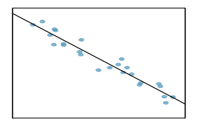
\includegraphics[width=2.08333in,height=\textheight]{images/img55.png}

Select the correct choice.

\emph{(a)} Strong positive relationship

\emph{(b)} Strong negative relationship

\emph{(c)} Weak positive relationship

\emph{(d)} Weak negative relationship

\textbf{Exercise 2}

The mean travel time from one stop to the next on the Coast Starlight is 129 minutes, with a standard deviation of 113 minutes. The mean distance from one stop to the next is 108 miles with a standard deviation of 99 miles. The correlation between travel time and distance is 0.636.

\emph{(a)} Write the equation of the regression line for predicting travel time (based on the distance).

\emph{(b)} Interpret the slope and the intercept in this context.

\emph{(c)} Calculate and interpret \(R^2\).

\emph{(d)} The distance between Santa Barbara and LA is 103 miles. Use this model to estimate the time it takes to travel between these two cities.

\emph{(e)} It actually takes the Coast Starlight about 168 minutes to travel between Santa Barbara and LA. Calculate the residual. Is the model over or underestimating the time?

  \bibliography{book.bib,packages.bib}

\end{document}
